% Created with jtex v.1.0.18
\documentclass{article}
\usepackage{arxiv}

\usepackage[utf8]{inputenc} % allow utf-8 input
\usepackage[T1]{fontenc}    % use 8-bit T1 fonts
\usepackage{hyperref}       % hyperlinks
\usepackage{url}            % simple URL typesetting
\usepackage{datetime}       % show dates in the title block
\usepackage{booktabs}       % professional-quality tables
\usepackage{amsfonts}       % blackboard math symbols
\usepackage{nicefrac}       % compact symbols for 1/2, etc.
\usepackage{microtype}      % microtypography
\usepackage{graphicx}
\usepackage{natbib}
\usepackage{doi}
\usepackage{xcolor}

%%%%%%%%%%%%%%%%%%%%%%%%%%%%%%%%%%%%%%%%%%%%%%%%%%
%%%%%%%%%%%%%%%%%%%%  imports  %%%%%%%%%%%%%%%%%%%
\usepackage{amsmath}
%%%%%%%%%%%%%%%%%  math commands  %%%%%%%%%%%%%%%%
\newcommand{\CRRA}{\rho}
\newcommand{\uFunc}{\mathrm{u}}
\newcommand{\cLvl}{\mathbf{c}}
\newcommand{\mLvl}{\mathbf{m}}
\newcommand{\yLvl}{\mathbf{y}}
\newcommand{\aLvl}{\mathbf{a}}
\newcommand{\Rport}{\mathcal{R}}
\newcommand{\bLvl}{\mathbf{b}}
\newcommand{\pLvl}{\mathbf{p}}
\newcommand{\DiscFac}{\beta}
\newcommand{\cFunc}{\mathrm{c}}
\newcommand{\vFunc}{\mathrm{v}}
\newcommand{\Alive}{\mathcal{L}}
\newcommand{\Ex}{\mathbb{E}}
\newcommand{\permGroFac}{\Gamma}
\newcommand{\permShk}{\psi}
\newcommand{\tranShk}{\theta}
\newcommand{\pZero}{\wp}
\newcommand{\tranShkEmp}{\xi}
\newcommand{\cNrm}{c}
\newcommand{\RNrm}{\mathcal{R}}
\newcommand{\aNrm}{a}
\newcommand{\mNrm}{m}
\newcommand{\Rfree}{\mathsf{R}}
\newcommand{\rfree}{\mathsf{r}}
\newcommand{\eprem}{\varphi}
\newcommand{\Risky}{\mathbf{R}}
\newcommand{\risky}{\mathbf{r}}
\newcommand{\bqstNrm}{e}
\newcommand{\lqdt}{\ell}
\newcommand{\h}{h}
%%%%%%%%%%%%%%%%%%%%%%%%%%%%%%%%%%%%%%%%%%%%%%%%%%


\hypersetup{colorlinks = true,
linkcolor = purple,
urlcolor  = blue,
citecolor = cyan,
anchorcolor = black}

\title{Life Cycle Modeling is (Almost) \\ Ready for Prime Time}

\newdate{articleDate}{26}{9}{2024}
\date{\displaydate{articleDate}}

\makeatletter
\let\@fnsymbol\@arabic
\makeatother

\author{Christopher Carroll\footnotemark[1]\\
Johns Hopkins University\\Econ-ARK\\\AND
Alan Lujan\\
Johns Hopkins University\\Econ-ARK\\}

% Uncomment to override  the `A preprint' in the header
\renewcommand{\headeright}{}
\renewcommand{\undertitle}{}
\renewcommand{\shorttitle}{}

%% Add PDF metadata to help others organize their library
%% Once the PDF is generated, you can check the metadata with
%% $ pdfinfo template.pdf
\hypersetup{
pdftitle={\@title},
pdfsubject={},
pdfauthor={\@author},
pdfkeywords={},
addtopdfcreator={Written in Curvenote}
}

\begin{document}
\maketitle
\footnotetext[1]{Correspondence to: ccarroll@llorracc.org}

\begin{abstract}
The `life cycle model' of optimal saving for retirement is familiar to anyone who has taken an introductory economics class.
When hiring a financial advisor, such people probably think the advisor's job is just to tailor optimal life-cycle-model choices to their particular circumstances.
But academics and advisors know that the advice about both saving and portfolio choice provided by standard academic life-cycle models is deeply problematic -- for example, most such models imply that retirees should plan to run their wealth down to zero or some small amount and then (optimally!) live pension-check to pension-check (at least approximately).
This paper makes the case that recent developments in the economics literature have finally given us the tools and insights required to construct rigorous life cycle models whose advice is sensible.
We provide one example of a simple model that can solve a number of problems by putting wealth in the utility function.
\end{abstract}

\keywords{}

% % [ ] AL: Remind me - we are now incorporating aggregate productivity growth of 1.5 percent/yr? look at Caggetti and figure this out
% % [ ] AL: Have we imported Mateo's medical expense risks yet? If so, delete this line, and make an "issue" in HARK that we should make that a default in our life cycle model indirect inference exercise (if we have not already done it)

\section{Introduction}

Franco Modigliani and Richard Brumberg (1954)\footnote{\cite{2005}} were the first to propose trying to understand consumer financial choices as optimal responses to the realities of the paths of income and of spending needs over the lifetime.
An enormous academic literature has followed their pioneering work (see the literature~appendix for an expansive summary),
but it has proven difficult to build rational optimizing models that give sensible advice about both life-cycle saving choices and about investment decisions.
That is, the models yield implausible answers to questions about how much wealth should be retained later in life, and how much of one's retirement savings should be invested in the stock market.
Indeed, the subtitle of a recent paper by \cite{Daga_2023} captures the current state of affairs nicely: ``Why Practitioners Have Not Adopted the Lifecyle Model -- Yet''; see also \cite{DeNardi2016d}.

In this paper, we argue that the elements are already available to construct a model that `practitioners can adopt,' and all that is needed is to combine the relevant academic contributions with some wisdom from practitioners' own experience of advising clients.
Our paper's central contribution is to provide a small \href{github.com/econ-ark/life-cycle-prime-time}{open-source computational model} that incorporates some of the features that make it possible to build rigorous optimizing life cycle models whose advice is not obviously wrong.

We begin with a (very) brief literature synopsis, then present a set of models that illustrate the difficulty of matching empirical facts with the life-cycle approach.
We end with our proposed solution, which involves a small twist to the old idea (\cite{carrollWhyDoTheRich}) of incorporating wealth directly in the utility function.

\subsection{Recent Developments in the Literature}

\subsubsection{Computation/Uncertainty/Complexity}

Consumers face many uncertainties: about their own income, stock returns, interest rates, health expenditures, mortality, and much more.
Further complications arise because of liquidity constraints and other financial frictions.

The incorporation of realistic descriptions of these complexities makes computation of the mathematically optimal solution to the consumer's astonishingly difficult.
It is more difficult than, say, the calculation of optimal trajectories for spacecraft, and perhaps comparable to the complexity of figuring out how to drive a car roughly as well as a human (another problem where adequate computational solutions have only recently become available).
The remarkable advance of computational power has now finally made it possible to compute a credible answer to the question ``what saving and portfolio choices are truly mathematically optimal?'' in a context where the key complexities are properly represented.

\subsubsection{Survey Data on Expectations and Preferences}

Another academic development has been a new openness to the idea that people's beliefs and preferences can be probed by \textit{asking them} about their beliefs and preferences.

In the context of motivations for saving, this leads us to take seriously the answers to a survey question about their `most important' reason for saving that respondents to the Federal Reserve's \href{https://www.federalreserve.gov/econres/scfindex.htm}{Survey of Consumer Finances (SCF)} have been asked for many years.
Among retirees, one answer dominates the rest: `Liquidity/The Future.'  (See the~discussion~below for details).

A natural interpretation of the importance consumers put on `liquidity' is that precautionary saving motives matter for many households -- highlighting the need for the aforementioned computational advancements.

The traditional approach to constructing such models has been for economists to try to measure the necessary inputs (income uncertainty, e.g.), and to assume that agent beliefs incorporate whatever it is that the economist has measured.
However, the newly collected survey data on consumer expectations show that the beliefs that many people {\textbackslash}textit\{actually\} hold differ substantially from what economists postulate they `should' believe based on their empirical measurements.
Moreover, there is now considerable evidence that the decisions people make reflect their actual beliefs and preferences rather than whatever it is that economists think they \textit{should} believe and prefer.\footnote{A particularly troubling possibility is raised by the work of \cite{gabaix2010age}, who point out that at least some elderly decision-makers (say, those with dementia) may be beyond the `age of reason.'}

% And, rather than being constant with age as economists typically assume, @albert2012differences provide evidence that risk aversion increases with age.

Some recent work suggests that taking beliefs data into account could resolve many of the problems that have long beset the life cycle modeling literature.
For example, \cite{velasquezgiraldoJMP} shows that even college-educated people systematically have held beliefs about stock market returns that are pessimistic compared to what the market has historically delivered.
He argues that this explains why people have been less eager to invest in stocks than would be predicted by models calibrated with economists' more optimistic expectations, and that the portfolio investment behavior of college-educated people over most of their lives is reasonably consistent with \textit{subjectively} rational decision-making (i.e. given their beliefs).
Concretely, many people think that investment in stocks is a lousy deal, yielding a low return with high risk, so it's no mystery why such people do not invest.

It is not astonishing to discover that many people hold beliefs that differ from those of experts, especially on subjects whose mastery requires considerable domain-specific education, like the returns and risk of stock investments.
Indeed, the existence of a large industry offering financial advice is \textit{prima facie} evidence that many people are not confident that they understand everything necessary to make good financial financial choices on their own.

Financial advice, however, is fraught with potential conflicts of interest.
That is one reason that justifying such advice with an explicit and transparent modeling framework is so attractive.
If the advice is consistent with the model, and the model can be checked both for mathematical correctness and conceptual soundness (by outside experts), then it is reasonable for a client hiring an advisor to trust the advice.

\subsubsection{Model Specification and Estimation}

In the Models section below, we provide a formal description of the mathematical and computational structure of our optimizing models, beginning with the Life~Cycle~Portfolio model, which calculates optimal saving and optimal portfolio shares over the life cycle.
In the Estimation, we report that the model implies a rapid drawdown of wealth after retirement that is simply not observed in empirical observations, confirming a longstanding problem with life cycle models (see, e.g., \cite{hurd1987savings}, \cite{HEIMER_2019}).\footnote{Some impressive recent work by Ameriks, Caplin, and coauthors (\cite{ameriks2011joy}, \cite{Ameriks2020jpe}) has argued that concerns about the possibility of extremely large medical costs (e.g. nursing home or other long term care) may be behind the drawdown failure for some people (see \cite{DeNardi2016d}) for a survey).}
We call this the `drawdown failure,' which has been the subject of a large literature with both U.S. evidence (see, e.g., \cite{Hurd_1989}, \cite{DeNardi2016d}, \cite{Kopecky_2014}, \cite{Mortenson_2019}, \cite{Poterba_2018}) and international evidence (see, e.g., \cite{Christensen_2022}, \cite{Ventura_2020}, \cite{Niimi_2019}).

% % Although our model attempts to take medical expenditure shocks into account, it is not calibrated directly with the @Ameriks2020jpe measurements of medical shocks in the US.

It would be interesting to see how our results might change if we were to include such shocks, but the inexorable logic behind the model's prediction of a rapid drawdown of wealth should still apply as the threat of mortality grows with age.
Furthermore, the drawdown failure is also present in other countries whose social insurance systems are much more generous than the U.S., so it seems unlikely that uninsurable medical risk is a sufficient explanation.

We next modify the model by adding a bequest motive, because the literature has extensively explored whether such a motive could explain the drawdown failure (\href{@deNardi2004}{}],\cite{DeNardi2016d}).
But in the Estimation section we confirm the consensus in the literature that the bequest motive does not seem to have much force for most households.
(Note that \cite{Hendricks_2002} finds that for the great majority of households, bequests amount to less than 2 percent of lifetime resources).

This leads us into more speculative territory.
If what consumers care most about is to hold wealth for `Liquidity/The Future' but that wealth is not explainable by precautionary saving against measurable shocks, a potential interpretation is that consumers value the ownership of wealth \textit{in and of itself}.
After fleshing out this idea a bit, we propose a final model that makes wealth a direct input to the utility function in a slightly different way than in the existing life cycle literature.

The main quantitative result of this paper is to show that this final model does a better job jointly matching the data on wealth profiles and portfolio choice than either the Life Cycle Portfolio or the Warm Glow Bequest models.
More broadly, our modeling and conceptual tools have recently advanced to the point where it is finally possible to construct rational optimizing models of life-cycle financial choice that can serve as a credible justification for normative advice.
In particular, these conceptual advances include the idea that ``softer'' data like surveys on household expectations and beliefs should be taken seriously.

But the broader point is that, recently, our modeling and conceptual tools (including the idea that softer data like surveys should be taken seriously) have advanced to the point where it is finally possible to construct rational optimizing models of life cycle financial choice that can serve as a credible justification for normative advice.

\section{Models}

The academic literature on life-cycle modeling is vast, and we cannot hope to do it justice (even in the broader sampling in the literature~appendix).
But the intrinsic nature of papers in any academic literature is to focus narrowly on one specific question at a time.
Here, our goal is to examine the ``big picture'' question of what elements are needed to craft a model that can provide credible advice to retirees about spending and portfolio choices, while remaining reasonably consistent with the relevant well-established facts from the academic literature, as well as one new kind of further evidence that we view as vital: the experience of financial advisors themselves in interactions with their clients.
We have been told,\footnote{Personal communication, James Tzitzouris with Christopher Carroll, 2024-05-15.} for example, that a good way to get fired as a financial advisor is to recommend the LCP model's conclusion that it is optimal for retirees to plan to run their wealth down to zero then live pension-check to pension-check.

For purposes like 401(k) or other pension plan design, the optimization problem should be constrained to be one that satisfies the legal obligations employers have to their employees.
For example, the employer's contract is with the employee, not with the employee's heirs.
The employer's duty is to craft a plan that is expected to permit the employee to have adequate resources for their own expenditures during retirement.
These legal considerations effectively prohibit the advisor from including a bequest motive in its optimization objective.\footnote{One way to accommodate this requirement would be to limit the empirical sample used to estimate the model to childless people.
This might not be feasible with public datasets like the SCF because the sample sizes might be too small; but with large administrative data of the kind available to 401(k) providers it should be possible.}

% % MNW: I undid the section labeling here because the edits generated a duplicate label. A single model is presented in this subsection, introducting the basic lifecycle first, then adding portfolio choice to close the model.

\subsection{The Baseline Academic Model}

We begin by describing the optimal consumption-saving problem over the life cycle for a consumer, focusing on the dynamics of their income while ignoring how returns to saving work.
After we have finished describing the basic life cycle model, we will augment it to add optimal portfolio choice between a safe asset and a risky asset (like the stock market) with a higher expected rate of return.

\subsubsection{Basic Life-Cycle Consumption-Saving}\label{basic-cs}

In each year (indexed by $t$), a consumer's flow of utility depends on how much they consume from their available resources.
We assume that the utility function is of the standard Constant Relative Risk Aversion form:
\begin{align}
    \uFunc(\cLvl) & = \frac{\cLvl^{1-\CRRA}}{1-\CRRA}.
\end{align}
The consumer is smart enough to realize that preserving some resources for the future is a good idea: they do not consume all of their wealth immediately.

% % MNW: Adjusted this sentence to make it complete.

At the time they choose how much to consume, the consumer has total market resources of $\mLvl_t$, representing their previously owned resources (bank balances) and current income flow $\yLvl_t$.
Whatever the agent does not consume constitutes assets $\aLvl_t$, which accrue interest by factor $\Rport_{t+1}$ between period $t$ and period $t+1$.
We follow most of the literature and assume that the consumer faces a hard liquidity (or borrowing) constraint: they cannot end any period with negative assets.
These assumptions are expressed as:
\begin{align}
    \aLvl_t = \mLvl_t - \cLvl_t, & \text{~~~remaining assets are market resources less consumption} \\
    \aLvl_t \geq 0, & \text{~~~consumer cannot borrow} \\
    \bLvl_t = \Rport_{t+1} \aLvl_t, & \text{~~~bank balances are assets after yielding interest} \\
    \mLvl_{t+1} = \bLvl_{t+1} + \yLvl_{t+1}. & \text{~~~future market resources are bank balances plus income} \\
\end{align}

One of the fundamental discoveries of the past 40 years or so is the extent to which optimal choice is profoundly altered by the presence of uncertainty.
\cite{friedman1957} proposed a simple formulation of the labor income process that remains an excellent description of annual income shocks even today.  According to Friedman, there are two components to income.
The `permanent' component is roughly what the consumer would expect to earn in a `normal' year (say, their annual salary), and a `transitory' component reflects events like unemployment spells or lottery winnings, which make a given year's realized income deviate from its expected value.
From a modeling perspective, the upshot is that a consumer's financial circumstances can be fully captured with two variables.
First, the consumer's permanent income level $\pLvl_{t}$ is the non-capital income they would normally expect to receive.
Second, total market resources $\mLvl_{t}$ represent the sum of financial assets and current income: the pool of resources that can be immediately spent, or `money' in the colloquial sense of `how much money does grandma have?'.
The transitory component of income need not be tracked at all: as soon as this uncertainty is resolved, its information is fully incorporated by market resources $\mLvl_{t}$.

A consumer's `value' of having a given amount of market resources $\mLvl_{t}$ right now, and of knowing their current permanent income level to be $\pLvl_{t}$, is the sum of consumption utility they will experience from today onward into the indefinite future, assuming that they make optimal choices in all periods.
Potential future utility flows matter only to the extent that the agent expects to survive to that period, and might be further discounted due to placing more weight on the present than the future.

In formal mathematical terms, the consumer's objective is to maximize expected present discounted utility from consumption over a life cycle that ends no later than some terminal period $T$:

\begin{equation}
\label{eq:lifecyclemax}
\pmb{\vFunc}_{t}(\mLvl_{t},\pLvl_{t}) = \max_{\{\cFunc\}_{t}^{T}} ~ \uFunc(\cLvl_{t})+\Ex_{t}\left[\sum_{n=1}^{T-t} \Alive_{t}^{t+n}{\DiscFac}^{n} \uFunc(\cLvl_{t+n}) \right].
\end{equation}
\begin{align*}
    \Alive _{t}^{t+n} & : \text{probability to } \Alive \text{ive until age $t+n$ given you are alive at age $t$}
    \\                   & {~~~}\bullet \Alive_{120}^{121} = 0.0 \text{ says that a 120 year old has zero probability of living to 121}
    \\                   & {~~~}\bullet \Alive_{80\phantom{1}}^{90\phantom{1}} = 0.3 \text{ says that an 80 year old has a 30 percent chance of reaching 90}
    \\ \DiscFac = 1        & : \text{time discount factor (captures degree of present bias)}
\end{align*}

To capture the predictable patterns that non-capital income follows over the life cycle (i.e. rising with age and experience, and falling at retirement to the level of any regular pension payments), we define a sequence to characterize the Modiglianian life cycle:
\begin{align}
    \permGroFac_{t+1} & : \text{typical life cycle permanent income growth factor by age}
\end{align}

The typical life cycle pattern is altered, in any particular consumer's case, by `permanent shocks' which we represent with the variable $\permShk$.
At any given age, permanent growth can deviate from the average experience of others of the same age in either a positive direction ($\psi>1$ would correspond to an unexpected promotion or a switch to a higher-paying job) or a negative direction ($\psi < 1$ might be the result of a failure to be promoted or a change to a lower paying job).

This gives us the following description of the dynamics of income:
\begin{align}
    \pLvl_{t+1} & = \pLvl_{t} \permGroFac_{t+1} \permShk_{t+1}, \\
    \yLvl_{t+1} & = \pLvl_{t+1} \tranShk_{t+1}, \\
    \Ex_{t}[\pLvl_{t+1}] & = \pLvl_{t} \permGroFac_{t+1},
\end{align}
where the third line follows because the expected value of the permanent shock is $\Ex_{t}[\permShk]=1$.

The transitory component $\tranShk$ of income has two modes.
In unemployment spells, the consumer earns no income; we assume that such spells occur with probability $\pZero$ each period.
Otherwise, the consumer receives a transitory income shock $\xi > 0$ from some (mean one) distribution, rescaled to preserve the unit mean of $\tranShk$:\footnote{It is straightforward to extend the model to allow for a more realistic treatment of unemployment, for example by taking account of the existence of an unemployment insurance system; such an adjustment does not change the substantive conclusions we are interested in.}
\begin{align}
    \tranShkEmp_{s} = &
    \begin{cases}
        0\phantom{/\pZero} & \text{with probability $\pZero>0$}
        \\ \xi_{s}/(1-\pZero) & \text{with probability $(1-\pZero)$}
    \end{cases}
\end{align}

It is conventional to assume that shocks to permanent income and to the transitory income of the employed are (mean one) lognormally distributed:
\begin{align}
    \log \permShk_{s} \sim \mathcal{N}(-\sigma_{[\permShk, t]}^{2}/2,\sigma_{[\permShk, t]}^{2})
    \\ \log \xi_{s} \sim \mathcal{N}(-\sigma_{[\xi, t]}^{2}/2,\sigma_{[\xi, t]}^{2})
\end{align}
which, together with the other assumptions, guarantee that the expected value of the transitory and of the permanent shocks are both 1: $\Ex_{t}[\permShk_{t+1}]=\Ex_{t}[\tranShk_{t+1}]=1$.
(We use standard calibrations of both of these shock processes.)

Under the assumptions we have made about the structure of the utility function (homotheticity), budget constraint (linearity and geometric returns), and income process (permanent and transitory shocks) it is possible to recast the problem entirely in terms of \textit{ratios} of the model variables to permanent income $\pLvl$.
So, for example, italic $\cNrm = \cLvl/\pLvl$ is the ratio of the (boldface) level of consumption to the level of permanent income $\pLvl$ (see \cite{BufferStockTheory} for the math).

Another way to make the problem easier to understand is to combine several of the multiplicative terms into portmanteau variables.
Particularly, define $\pmb{\DiscFac}_{t+1}$ as
\begin{align}
     \pmb{\DiscFac}_{t+1} & ={\beta} (\permShk_{t+1} \permGroFac_{t+1})^{1-\CRRA}.
    %\\ \RNrm_{t+1} & = \left(\frac{\Rport_{t+1}}{\permShk_{t+1}\permGroFac_{t+1}}\right)
\end{align}

% and simplifying the notation for the probability of survival to $\Alive_{t+1} \equiv \Alive_{t}^{t+1}$

The consumer's problem can be expressed more simply by realizing that it boils down to a ``now versus later'' problem.
All the consumer needs to know about the future is summarized by the value they will expect as a consequence of ending the current period with a certain ratio of assets to permanent income, $\aNrm = \aLvl/\pLvl$.
We can represent the value of ending the period with assets of $\aNrm_t$ using the Gothic variant of the letter $\vFunc$:
\begin{align}
    \mathfrak{v}_{t}(\aNrm_{t}) & = \Ex_{t}[\pmb{\DiscFac}_{t+1}\vFunc_{t+1}(\mNrm_{t+1})].
\end{align}

With this definition, the period $t$ choice problem can be summarized in Bellman form as simply:
\begin{equation}
\vFunc_t(\mNrm_t) = \max_{\cLvl_t} \left\{ \uFunc(\cLvl_{t}) + \Alive_{t+1} \mathfrak{v}_{t}(\aNrm_{t}) \right\} = \max_{\cLvl_t} \left\{ \uFunc(\cLvl_{t}) + \Alive_{t+1} \mathfrak{v}_{t}(\mNrm_{t} - \cNrm_t) \right\}.
\end{equation}
Because $\aNrm_t$ measures available market resources that are unspent, this formulation makes it crystal clear that the consumer faces a tradeoff between the utility of consumption today and the expected value of preserving assets $\aNrm=\mNrm -\cNrm$ for the future.\footnote{The normalization for value function involves more than just division by $\pLvl$; see \cite{BufferStockTheory} for details.}

\subsubsection{The Life Cycle Portfolio (`LCP') Model}\label{lcp-model}

We are now ready to add portfolio choice to the problem and discuss how the interest factor $\Rport_{t+1}$ is determined.
Suppose the consumer can invest their assets in a risk-free asset with return factor $\Rfree$, and in a risky asset with returns $\log \Risky_{t+1} \sim \mathcal{N}(\rfree + \eprem - \sigma^{2}_{\risky}/2, \sigma_{\risky}^{2})$, where $\rfree = \log(\Rfree)$.
That is, we make the conventional assumption that risky returns are lognormally distributed with an expected equity premium of $\eprem$.
The portfolio return the consumer earns will depend on the \textit{share} $\varsigma_t$ of their assets that they invest in the risky asset:
\begin{align}
    \Rport_{t+1} & = \Rfree + (\Risky_{t+1}-\Rfree)\varsigma
\end{align}

Now the consumer makes \textit{two} choices in each period $t$: how much to consume $\cNrm_t$ and the share $\varsigma_t$ of his assets to put into the risky asset.
These choices are made simultaneously, but they can be thought of as being made sequentially, one immediately after the other: first consumption (conditioned on market resources $\mNrm_t$) and then the risky asset share (conditioned on assets $\aNrm_t$ after consumption).
The consumer makes the optimal choice of portfolio share, so we redefine the ``gothic'' value function as:
\begin{align}
\mathfrak{v}_{t}(\aNrm_t) & = \max_{\varsigma_t}~~ \Ex_{t}\left[ \pmb{\beta}_{t+1} \vFunc_{t+1}(\Rport_{t+1} \aNrm_t + \theta_{t+1}) \right].
\end{align}
A split second before choosing the risky share, the consumer's objective in the consumption stage of the problem is exactly the same as the Bellman form above, but with the redefined continuation value that accounts for optimal portfolio choice.

\bigskip\noindent
\begin{tabular}{p{\dimexpr 0.500\linewidth-2\tabcolsep}p{\dimexpr 0.500\linewidth-2\tabcolsep}}
\toprule
object & meaning \\
\hline
$\mNrm, \cNrm, \aNrm$ & market resources, consumption, and end-of-period assets, normalized by permanent income \\
$\vFunc$ & the normalized value function \\
$\Alive_{t+1} \equiv \Alive_{t}^{t+1}$ & probability that a person alive at age $t$ survives to age $t+1$ \\
\bottomrule
\end{tabular}

\bigskip
% {and} since $\aNrm$ measures available market resources that are unspent, this formulation makes it crystal clear that the consumer faces a tradeoff between the utility of consumption today and the expected value of preserving assets $\aNrm=\mNrm-\cNrm$ for the future.[^normalization]
% % MNW: This deletion was mistakenly reversed, I think. This sentence was moved up to just before the subsubsection break.

\subsubsection{Calibration}

Many of the parameters of the basic life-cycle consumption-saving model can be calibrated from well measured empirical data.
For example, we use standard calibrations of both of the income shock processes during the working life, based on \cite{Cagetti2003}, and
survival probabilities by age are taken directly from actuarial mortality tables published by the Social Security Administration.
We set the `pure' rate of time preference to $\beta=1$, meaning that the optimal choice is to care exactly as much your future self as much as your present self (conditional on surviving into the future).

Beyond those basic assumptions, we calibrate the model to include two kinds of uncertainty after retirement.
First, to address the possibility that the drawdown failure reflects a fear of medical expenses, we incorporate estimates from \cite{velasquezgiraldoJMP} of the size of shocks to medical expenditures for retirees.
Our estimation results show that even when we include this calibration of medical shocks, the model still predicts much more drawdown of wealth than the data show.
Second, we assume that there are `ordinary' expenditure shocks in retirement that are of similar magnitude to income shocks during working life (following recent estimates from  \cite{flExpShocks}).
Again, in principle, the presence of such shocks provides a precautionary motive to draw down wealth more slowly.

\subsection{Alternative Preferences}

The specification of preferences in the LCP model is the standard assumption of time-separable Constant Relative Risk Aversion.
This is the workhorse tool for intertemporal choice models because it has a number of convenient mathematical properties and its implications satisfy some plausible economic desiderata (cf. \cite{kimballStandardRA}).
However, mathematical convenience provides no guarantee that the utility specification is \textit{right} in the sense of giving a proper representation of what people's preferences really are.
Economists have explored a number of modifications to these standard preferences in an attempt to make their models' predictions match various facts.

\subsubsection{Habit Formation and Epstein-Zin Preferences}

One intuitive idea is that people care not only about the current level of their consumption but also about how it compares to their past levels of consumption (they have ``habit formation'' in their preferences).
For example, \cite{Carroll_2000} show that a model with multiplicative habits can provide an explanation for otherwise puzzling patterns in the relationship between saving and growth across countries, and
\cite{Michaelides_2002} examine the implications of such a model for life-cycle choices.

A second common modification to preferences considered by a substantial literature is the use of \cite{Epstein_1991} preferences, which allow agents to be extremely risk averse with respect to financial risk at a point of time, while simultaneously allowing the agents to be willing to be quite willing to tolerate changes in consumption over time.
Such preferences have been proposed as a way to solve various puzzles related to the relatively high rate of return that equity investments have exhibited over time.

Both of these formulations are motivated mostly by the goal of matching macroeconomic data.
In our view, however, they are both difficult to defend given some facts we can robustly observe in microeconomic data.
In particular, both models would imply that microeconomic households would be extremely eager to buy insurance to smooth away almost any risk to their microeconomic circumstances.
While people do typically have insurance against large risks (fire insurance for the home, auto insurance for the car), the parameter values in these models required to match the macroeconomic facts would justify consumers in spending a large fraction of their income on insurance of all kinds.
One particular example stands out: Households with either strong habits or a high Epstein-Zin instantaneous coefficient of relative risk aversion would be extremely eager to buy private unemployment insurance to supplement the default UI system provided by the state.
Indeed, such private UI is available-- and at prices such that a large fraction of households would be eager to buy it if they had such preferences-- yet the fraction of households who participate in the private UI market is vanishingly small.

Our attention in this paper is therefore directed toward other modifications in preferences that seem to be plausible in both microeconomic and macroeconomic data.

\subsubsection{The ``Warm Glow'' Bequest Motive}

The LCP model sketched above assumes that the only reason to hold wealth is to spend it later, which means that eventually an age must come at which the wealth starts being spent down.
As the literature has demonstrated, and as we will confirm below using data from SCF's from 1995 to 2022, the path of the median wealth ratio after retirement does not look anything like what that model predicts.

Of course, the model can make no sense at all of the behavior of the very rich.
Bill Gates, for example, has chosen to allocate a large portion of his lifetime wealth to the Bill and Melinda Gates foundation rather than spending it on himself; and even with the relative pittance that remains to him (\$153 billion, per \href{https://www.businessinsider.com/how-bill-gates-spends-fortune}{Business Insider}) he would need to spend about \$22 million per day to \textit{avoid getting richer}.\footnote{As of 2024-05-15, the Fed Funds rate is 5.3 percent at an annual rate.
\$153b $\times$ 0.053/365 days $\approx$ \$22 million.
At the current inflation rate of 3.4 percent, he would only have to spend a little over \$8 million a day to run down his real wealth -- assuming the Fed Funds rate is the highest rate of return he can earn.}
In fact, he has pledged to give away nearly all of his wealth before he dies.

But the model also fails for people of much more modest means - the `drawdown failure' articulated above.
From a mathematical point of view, it is clear that some other motive for holding onto wealth must be added to the framework if it is to explain the broad facts, never mind Bill Gates.
A natural candidate is a bequest motive: The idea that people take pleasure in the thought of leaving something to their heirs.

This idea can be incorporated by adding another term to the sources of utility: the value the consumer places on the bequest, which we will denote as $\bqstNrm(\aNrm)$, the utility they experience from the thought of leaving an $\bqstNrm$state.
The flow of utility that the consumer receives includes both their utility from consumption \textit{and} the pleasure they take from the thought that, if they pass away before next period (which happens with probability $1 -\Alive$), their assets will pass to their heirs.

The consumer's new value function is therefore:
\begin{align}
    {\vFunc}_{t}({\mNrm}_{t}) & = \max_{\cNrm_{t}} ~ \overbrace{\uFunc(\cNrm_{t})}^{\text{present}}+\overbrace{\underbrace{\Alive_{t+1}\mathfrak{v}(\aNrm_{t})}_{\text{live}} + \underbrace{(1-\Alive_{t+1})\bqstNrm({\aNrm}_{t})}_{\text{die}}
    }^{\text{future}}.
\end{align}

The literature has commonly used a `warm glow utility from bequests' motive of the form:
\begin{align}
    \bqstNrm(a) & = \alpha\frac{(a+\underline{a})^{1-\CRRA}}{1-\CRRA}
\end{align}
where the $\CRRA$ coefficient is the same as in the utility function for consumption (see, e.g., \cite{deNardiBequest}), and the $\alpha$ coefficient controls the importance of the bequest motive relative to the utility from consumption.

Our estimation finds little evidence that a bequest motive of this kind is important for the median college-educated retiree.
It also seems unlikely to be important for much richer people, at least according to the evidence from the historian Fredrick Cople \cite{jaherGilded}'s chronicle of the behavior of the richest Americans since the Revolution.
Jaher presents a feast of quotations articulating a host of motivations for extreme wealth accumulation; but among their many explanations of their behavior, almost none of the tycoons under study mention anything resembling the bequest motive as formulated in the standard academic life cycle literature.
Andrew Carnegie was most explicit: `I would rather leave my son a curse than the almighty dollar.'\footnote{He made good on this: He gave away more than 90 percent of his wealth before he died, to the astonishment of many skeptics.}

As mentioned above, the \cite{2023} has for many years asked respondents a question about their motivations for saving.\footnote{See the material starting at line 848 in \href{https://www.federalreserve.gov/econres/files/bulletin.macro.txt}{the documentation}.}
While respondents' answers are fairly heterogeneous, the SCF has a suggested aggregation of the many different answers into categories that correspond approximately to some of the motivations that the academic literature has considered.
The category that best matches the `bequest' motivation is `Family' (which includes `to help the kids out' and `to leave an estate' but also includes saving for `weddings and other ceremonies' and `to have children/a family.')

An ambitious agenda would be to tabulate the answers to this survey question for people at different ages and then to construct a model that would imply the same age pattern of motivations as the data.
For example, one might find that for people who have just entered the labor market (say, the 26-30 age group) the survey responses showed that saving for `retirement' was not a priority, while saving for `purchases' and `liquidity' were important.
In order for a model to be credible, its implications would need to comport with the survey data.
Our aim here is to take a first step in that direction, by constructing a model that is at least consistent with the responses of retirees.

The table below presents the responses to this question for college-educated households older than age 70 from the 1995 to the 2022 waves of the SCF.
If bequests were a primary motivation for saving for most (college-educated) people, it would be surprising for them to mention this motivation so rarely.
Given these (and other) objections to the bequest motive, as well as the problems of the model without a bequest motive, it is natural to consider alternative modifications to the framework.

\subsubsection{Table: Most Important Reason for Saving}\label{most-important-reason}

\bigskip\noindent
\begin{tabular}{p{\dimexpr 0.333\linewidth-2\tabcolsep}p{\dimexpr 0.333\linewidth-2\tabcolsep}p{\dimexpr 0.333\linewidth-2\tabcolsep}}
\toprule
Reason & Proportion & Explanation \\
\hline
`Family' & 0.06 & bequests; weddings, etc \\
`Retirement' & 0.27 &  \\
`Liquidity/The Future' & 0.40 &  \\
`Purchases' & 0.13 & cars, vacation homes, etc \\
`Cannot save' & 0.06 &  \\
Other & 0.08 &  \\
\bottomrule
\end{tabular}

\bigskip\subsection{Wealth in the Utility Function}

Explaining the motivation to save is one of those places where economists' new openness to the idea of taking seriously what people say about their motivations has bite.
While it is reasonable to be skeptical about taking quotations from \cite{jaherGilded} at face value, \cite{WhyDoTheRich} shows that essentially all of the motivations articulated (wealth brings power; wealth allows philanthropy; wealth is a way of `keeping score'; and more) can be captured in a mathematical formulation in which wealth enters the utility function directly.

The most general way that economists have for incorporating people's motivations into models of behavior is simply to assume that the decision-maker directly values something -- in this case, wealth.
The question is how best to incorporate the item in the utility function to study any particular question.
\cite{WhyDoTheRich}, for example, proposed a utility function specifically designed to capture saving behavior as wealth approached infinity, and accomplishing that goal required some mathematical structure that delivered the desired results but was unwieldy (and not obviously necessary for explaining the behavior of the bottom 99 percent, whose wealth does not approach infinity).\footnote{Specifically, a separable utility-from-wealth function was added to the maximizer's objective and with a coefficient of relative risk aversion smaller than that for the utility from consumption.}

\subsubsection{Money in the Utility Function}

There is a literature in macroeconomics, pioneered by Miguel \cite{sidrauski1967rational}, that has long included `money' (in the monetary sense) in the utility function of the representative agent in one form or another.
A well-known paper by \cite{Rotemberg1984} proposed a specific utility function designed to capture the stability of the ratio of money to GDP, and Rotemberg along with James Poterba estimated this model on U.S. data in \cite{Poterba_1986}.

The structure of their utility function is
\begin{align}
    \uFunc(\cNrm,\lqdt) & = \frac{\left(
        \cNrm^{1-\delta}\lqdt^{\delta}
        \right)^{1-\CRRA}}{1-\CRRA}
\end{align}
where $\lqdt$ captures the the $\lqdt$iquidity services provided by money-holding.

To be clear, the aim of that literature was to explain the holding of $\lqdt$ defined as dollar cash holdings, to study questions like the `velocity' of money and the role of money supply and money demand in determining interest rates -- not to explain saving behavior.

\subsubsection{Wealth In the Utility Function: Cobb-Douglas Form}

But for the question of how to incorporate wealth in the utility function, \cite{Tzitzouris2024} proposed a mathematically identical formulation in which assets $\aNrm$ takes the place of $\lqdt$ in the Rotemberg-Poterba utility function.\footnote{The question of whether $\aNrm$ or $\mNrm$ should be in the utility function is of little importance; here we prefer $\aNrm$ because assets after consumption are immune to considerations of whether the time period is a year, a quarter, or a month.}
The Cobb-Douglas functional form is commonly used in other contexts, but does not seem to have been explored as a formulation for how to put a direct wealth-holding motive in the utility function.

% AL: Add citation to the 1998 paper you found

The upshot is that if we credit the proposition that the ownership of wealth yields utility, then there is good precedent for the functional form of \cite{Tzitzouris2024}.
Henceforth we will call this the Tzitzouris-Rotemberg-Poterba or `TRP' utility function.
It is a relatively simple matter to solve the revised problem with wealth in the utility function using the TRP utility specification. The revised utility and value functions of the problem are:
\begin{align}
    \uFunc_t(\cNrm_t, \aNrm_t) & = \frac{\left(\cNrm_t^{1-\delta}\aNrm_t^{\delta}\right)^{1-\CRRA}}{1-\CRRA}, \\
    {\vFunc}_{t}({\mNrm}_{t}) & = \max_{\cNrm_{t}} ~ \uFunc(\cNrm_{t}, \aNrm_{t})+\Alive_{t+1}\mathfrak{v}_{t}(a_{t}).
\end{align}

% % We refrain from a description of the solution methods here because they are documented in the accompanying code archive which fully reproduces all our results.

We are open to the possibility that wealth in the utility function is a reduced form for other motivations -- indeed, that was the thesis of \cite{WhyDoTheRich}.
In particular, the fact that in our SCF table above, `Liquidity/The Future' is the most popular answer among retirees for the most important reason to save might signal that the forms of uncertainty that we can measure -- like the \cite{Ameriks2020jpe} calculations about nursing home expense risks -- constitute only a fraction of the matters retirees might worry about.
Maintaining a buffer stock of wealth to protect oneself against `unknown unknowns' is possibly perfectly rational, and also nearly impossible to calibrate in a quantitative model in which we would need to have an accurate representation of people's beliefs about the magnitude, frequency, and persistence of `unknown unknowns.'
Even if you knew those answers, they would be, at best, `known unknowns.'

\subsection{Comparisons to Other Models Familiar to Practitioners}

\cite{Gordon_2014} in ``The Journal of Retirement,'' asserted that financial planning practitioners mostly used rules of thumb and heuristics to provide their advice.
That paper aimed to introduce the key concepts of formal life-cycle modeling to the audience of practitioners.
Since its publication, there appears to have been considerable movement in the direction advocated by its authors.
A number of leading financial institutions have made available partial descriptions of proprietary life cycle models that they are developing.
For this report, we decided to describe only models that have been published in peer-reviewed journals and whose detailed characteristics are knowable.

\cite{Daga_2023} looks at the post-retirement period and normalizes all variables by retirement income, but it does not incorporate risk to permanent income (as we do), nor does it attempt to reconcile post-retirement with pre-retirement behavior.
The model uses an additive utility of bequest with no shifter term, which has the implication that even income-poor households have a powerful bequest motive.
The multigoal framework additionally disaggregates consumption expenses into different categories, each with the same CRRA coefficient.
This reduces the effect of the diminishing marginal utility of consumption, such that the sum of utilities of consumption is greater than the utility of the sums of consumption.
Moreover, each goal has an allocation coefficient (relative importance) that is set subjectively by the researchers.

\cite{O_Hara_2015} incorporate an additively separable utilty of bequest like the bequest motive we explored above, and like our models it incorporates both permanent and transitory shocks to income.
However, the model uses Epstein-Zin preferences (see our above objections to this feature).
Their model also assumes that there is no uncertainty (except for mortality) in the post-retirement period, because that assumption has the convenient implication that the post-retirement period is extremely simple; the portfolio share, in particular, should remain constant at the infinite-horizon Merton-Samuelson solution.

\cite{Lanski_2022} uses a life-cycle consumption and portfolio choice model without any consideration of bequests like the one discussed above (although other aspects of the model are simpler than our specification).

There have also been publications that partake of the mathematical flavor of life cycle modeling but do not use the intertemporal choice framework.
\cite{Idzorek_2023} uses a static model of portfolio optimization, where the objective is to maximize the mean-variance trade off of a portfolio position with additional features such as non-pecuniary benefits.
Because this model is not dynamic, it can not consider and/or anticipate risks such as future market volatility, changes in preferences over the life cycle, mortality, and retirement horizon.

\section{Estimation}

\subsection{Indirect Inference Described}

Even if one knew all the parameters of the model (the consumer's coefficient of relative risk aversion, etc), solving an optimization problem that includes the many real-world complications described above (especially those due to uncertainty) is such a formidable problem that it only became possible about 25 years ago (and solving the models took days).

But of course we do not know the best values to choose for unobservable parameters like relative risk aversion and time preference rates.
The increasingly standard approach to this problem is the method of `indirect inference.'
Essentially, this means specifying the structure of your model except for the values of parameters that you cannot measure well (like time preference and risk aversion), and asking a numerical search algorithm to seek the values of those parameters that lets the model fit the data as well as it is capable of doing.
This requires the computer to solve the problem perhaps thousands of times, which is why indirect inference has only begun to come into its own recently, as computer speeds have become fast enough to tackle the problem.

\subsection{Indirect Inference Implemented: the Method of Simulated Moments}

We are particularly interested in finding the optimal post-retirement choices, both for the rate of spending and for portfolio allocation between safe and risky assets.
The method of simulated moments consists of finding the parameters that make the model's simulated moments (statistics), like the median wealth and the median portfolio share, match the corresponding empirical facts as closely as possible.

Consider an empirical moment $q_i$ where $i \in \{1,...,N\}$ and the corresponding simulated moment $\hat{q}_i(\theta)$, where $\theta$ is the vector of parameters that we are interested in estimating.
By solving and simulating our structural model with different $\theta$ parameters, we can calculate the simulated moments $\hat{q}_i(\theta)$ for each parameter set.
The method of simulated moments then consists of searching for the parameter set $\theta$ that minimizes the distance between the simulated versus empirical moments.
This is done by minimizing the following objective function:
\begin{equation}
\min_{\theta} \sum_{i=1}^{N}  \left( \omega_i [q_i - \hat{q}_i(\theta) ] \right)^2
\end{equation}
Here, $\omega_i$ is the weight of each moment in the objective function, representing the relative importance of each moment in the estimation process.
For example, we might be more interested in matching the median wealth than the median portfolio share, and thus assign a higher weight to the former.

For our exercise, we are interested in matching the median wealth to income ratios throughout the life cycle, and the median portfolio share of risky assets after retirement.
Because aggregate age data can be noisy and subject to selection bias and measurement error, we will aggregate the data into 5-year age bins to smooth out the noise and reduce the impact of selection bias.
Starting at age 25, we calculate the median wealth-to-income ratio as follows: Wealth is defined as the sum of all assets and liabilities, including financial assets, housing, vehicles, and debt.
For income, we use the sum of all wages, salaries, Social Security, and retirement income, excluding capital gains and other non-recurring income.
We then calculate the wealth to income ratio of every household in the age bin and remove households with an income of zero.
The median wealth-to-income ratio is calculated from the remaining households.
Because the SCF data is increasingly sparse at older ages, the raw empirical moments show a ``zig-zag'' pattern above age 75 due to the small sample size.
We smooth this out by holding the wealth-to-income ratio at 10.0 in the top three age brackets, the approximate mean among them.

In our structural model, we hard-code retirement to occur at age 65, whereas in the data we observe retirement at different ages, but predominantly between ages 60 and 70.
Therefore, we avoid the data for ages 60 to 69 to prevent any bias in the estimation process, but keep the data for ages 70 and above to capture the behavior of retirees.
Similarly, we calculate the median portfolio share of risky assets after retirement for ages 70 and above given by \cite{Aboagye2024}.

Considering the selection of moments we have chosen, it is clear that there is an imbalance between the wealth-to-income moments and the portfolio share moments.
There are more wealth to income moments than portfolio share moments (12 vs 5), and the portfolio share moments lie between 0 and 1, whereas the wealth to income ratios can be much larger.
To account for this, we set the weights to normalize the wealth to income ratios by the highest ratio in the data, making them all lie between 0 and 1, and adjust the weights for the portfolio share moments by a factor of 12/5, so that the two sets of moments are about equally weighted in the estimation process.
This ensures that our estimation process puts even weight on the two sets of moments, despite the difference in scale and number of moments.

Having chosen the moments we are interested in matching and their respective weights, we can now proceed to a discussion of estimating the parameters of our various models.
We use the \texttt{Econ-ARK} project's \texttt{HARK} package to solve and estimate the models, and \texttt{optimagic} (\cite{Gabler2022}, formerly \texttt{estimagic}) to perform the estimation process.
Our exercise consists of estimating one parameter (the coefficient of relative risk aversion) for the Life Cycle Portfolio Choice Model and up to three parameters (CRRA, the weight of the bequest motive, and the wealth shifter of the bequest motive) for the \texttt{LCP+WarmGlow} model, so we develop a robust and efficient estimation process that can handle a varying number of parameters. 
%  % We call the merging of features from the `HARK` and `estimagic` packages `Estim-ARK`.

Our estimation process is computationally expensive, requiring the solving and simulation of the model given a parameter set many times.\footnote{Because our simulated moments indeed require simulation, our moment generating functions $\hat{q}_i(\theta)$ have no analytical derivatives with respect to the parameters, so we must rely on numeric differentiation and clever optimization algorithms to find the optimal parameter set.
We use the \texttt{tranquilo} algorithm (\cite{Gabler2024}), which stands for TrustRegion Adaptive Noise robust QuadratIc or Linear approximation Optimizer, to find the optimal parameter set.
The \texttt{tranquilo} optimizer has many attractive features, such as being able to evaluate the function in parallel and estimate even noisy objective functions with many parameters, as well as being especially designed for least squares problems, such as the MSM.}

\subsection{Indirect Inference Results}

Table~\ref{parameters} shows the results of our estimation exercise, and the fit of the three estimated models is plotted below, in Figure~\ref{medwealth} and Figure~\ref{medshare}.

\begin{table}
\centering
\caption[]{Estimated parameter values for the life-cycle, warm-glow, and TRP / WIUF portfolio models.}
\label{parameters}
\begin{tabular}{p{\dimexpr 0.167\linewidth-2\tabcolsep}p{\dimexpr 0.167\linewidth-2\tabcolsep}p{\dimexpr 0.167\linewidth-2\tabcolsep}p{\dimexpr 0.167\linewidth-2\tabcolsep}p{\dimexpr 0.167\linewidth-2\tabcolsep}p{\dimexpr 0.167\linewidth-2\tabcolsep}}
\toprule
Name & Criterion & CRRA ($\CRRA$) & Wealth Share ($\delta$) & Bequest Factor ($\alpha$) & Bequest Shifter ($\underline{a}$) \\
Life-Cycle Portfolio & 0.821 & 8.039 &  &  &  \\
Warm-Glow LC Portfolio & 0.044 & 4.649 &  & 8415.7 & 2.588 \\
TRP / WIUF LC Portfolio & 0.250 & 4.883 & 0.159 &  &  \\
\bottomrule
\end{tabular}
\end{table}

For the standard Life-Cycle Portfolio (LCP) model, we estimate a CRRA $\CRRA$ coefficient of about 8, which lines up with the literature finding that portfolio choice models require a very high $\CRRA$ in order to prevent agents from putting all their assets in the risky form.
For context, ``typical'' values for the CRRA coefficient (from experimental evidence and other contexts) are considered to be between 1 and 5.
The ``criterion'' column of Table~\ref{parameters} lists the minimum value that the objective function achieves for each model-- the smallest weighted squared distance between simulated moments and empirical moments.
The LCP model performs poorly by this measure, as illustrated in the figures.
LCP consumers want to quickly run down their wealth at older ages, as the probability of death increases with age and they know that they ``can't take it with them''.
To try to match the observed empirical wealth trend (red dashed line in Figure~\ref{medwealth}), which holds steady at a high wealth-to-income ratio at older ages, the LCP model (solid blue line) exceeds observed wealth accumulation through the working life.
Even then, the wealth drawdown is so rapid that the best the LCP model can achieve is to significantly overshoot wealth before age 65, and then vastly undershoot it in retirement.

\begin{figure}[!htbp]
\centering
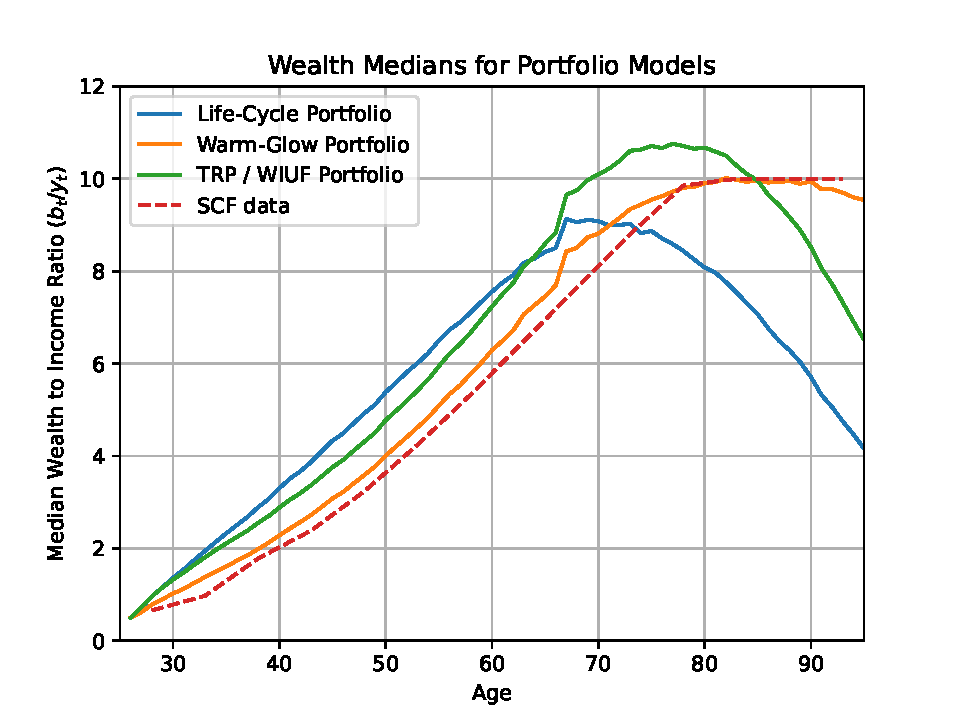
\includegraphics[width=0.7\linewidth]{files/median_wealth-d2524c71e6344dd7c4922a55ce47bf79.pdf}
\caption[]{Median Wealth to Income Ratio for different portfolio models. The red line indicates median wealth-to-income ratios for College educated households in the Survey of Consumer Finances. Wealth is \texttt{networth} and income consists of wages, social security, and retirement income.}
\label{medwealth}
\end{figure}

As discussed above, there are multiple model features that can ameliorate or eliminate the wealth drawdown problem, beginning with a simple bequest motive.
The Warm-Glow Portfolio model (orange lines on figures) estimates a much more realistic CRRA coefficient of $\CRRA = 4.65$.
With a strong bequest motive ($\alpha \approx 8400$), the Warm-Glow model is able to match the high levels of wealth observed deep into retirement.
That is, these consumers do not quickly draw down their assets because they take great pleasure in passing their estate on to their heirs.
The bequest motive magnitude $\alpha$ and shifter term $\underline{a}$ are somewhat complicated to interpret, but the upshot is that the bequest motive applies for essentially \textit{everyone}.
In contrast, the literature has generally found (e.g. \cite{deNardiBequest}) that the bequest motive comes into play only for relatively wealthy households, and is mostly inoperative around median wealth.
This discrepancy might arise because of the simplified approach we have used here, matching \textit{only} the median wealth-to-income ratio by age, rather than wealth levels conditional on income.

Digging deeper, the Warm-Glow model predicts that saving behavior \textit{when young} is strongly motivated by the bequest motive.
Recall from the discussion of the \cite{2023} and \cite{jaherGilded} that very few older people ascribe their wealth-holding behavior to a bequest motive, and yet the Warm-Glow model has the saving choices of \textit{40 year olds} driven by the urge to bequeath.
Even if a model can \textit{mechanically} reproduce observed data features or hit empirical targets, that does not make it ``right'' or ``true'', especially if its underlying logic is implausible and contradictory to qualitative evidence.
And as discussed above, the bequest motive is inconsistent with an investment advisor's fiduciary duty \textit{to the client}.
We include the Warm-Glow model in our presentation not to advocate for it, but merely to demonstrate that there are \textit{multiple ways} for life-cycle models to generate more realistic wealth trajectories in retirement.

\begin{figure}[!htbp]
\centering
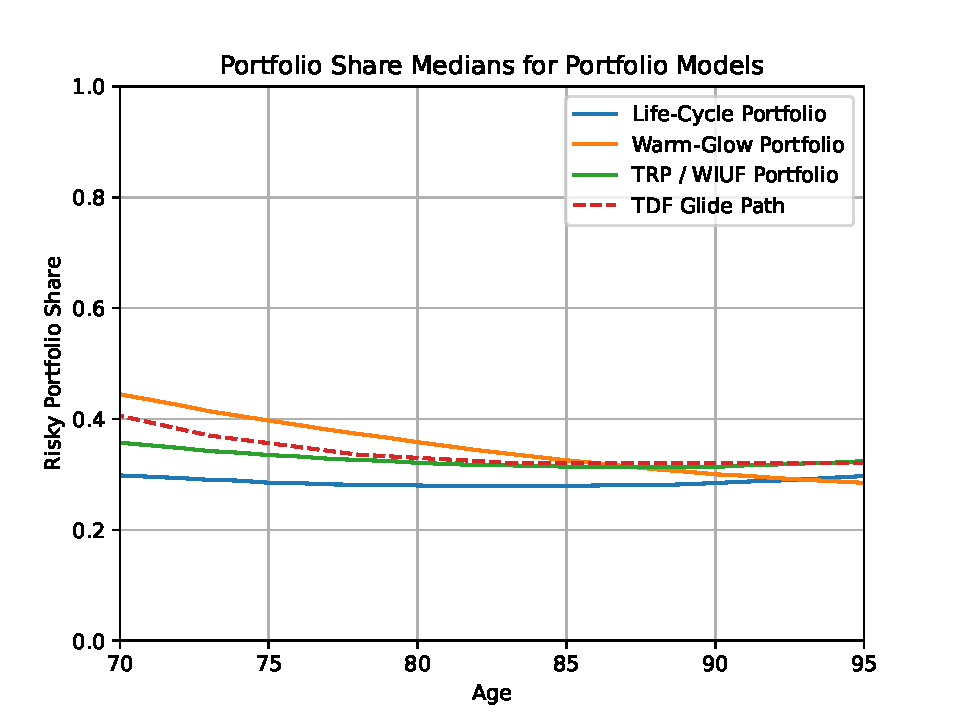
\includegraphics[width=0.7\linewidth]{files/median_share-375a692fb3207501be3ba379fe1a09eb.pdf}
\caption[]{Median Portfolio Share for different portfolio models. The red line shows the target moments from \cite{Aboagye2024}.}
\label{medshare}
\end{figure}

Our preferred specification also has the agents value wealth itself as a motivation to retain assets later in life, but in a way that is more consistent with qualitative responses.
The Wealth-in-Utility-Function (WIUF) / TRP Portfolio model estimates a CRRA $\CRRA$ coefficient of about 4.88 and a wealth share of utility $\delta$ coefficient of 0.16.
This result is significant because the CRRA $\CRRA$ coefficient required to match the wealth accumulation patterns is significantly lower than that of the Standard Life-Cycle Portfolio choice model, whose high CRRA $\CRRA$ has long been a puzzle in the literature.
As seen in Figure~\ref{medwealth}, the WIUF / TRP model (green line) does not need to overshoot wealth accumulation in early life by nearly as much as the basic LCP model, as agents want to retain assets in retirement to generate utility directly.
Compared to the Warm-Glow model, the TRP specification does predict more wealth accumulation early in life, but for more immediate reasons: young consumers value money and liquidity \textit{now}, rather than planning at age 35 to leave a large bequest at age 80.

Moreover, because the CRRA parameter doesn't need to be so high, the WIUF model can more accurately match the target risky assets share moments (red dashed line in Figure~\ref{medshare}), which come from \cite{Aboagye2024}.
That paper presents the typical glide-path of target-date funds (TDFs) which provide a basis for much of commercial financial advice.
While the whole life-cycle glidepath is provided in \cite{Aboagye2024}, here we only target (and plot) those moments starting at age 70.
The model fit with respect to risky asset share is comparable for the Warm-Glow model, generally matching the level and recommended shallow downward slope.
The basic LCP model, however, badly fits the risky asset share too low due to the high $\CRRA$ value needed in its attempt to match the life-cycle wealth pattern.

\section{Conclusion}

To thoughtful academics, it has long been disturbing that the financial advice industry has paid so little attention to our hard work in constructing and solving impressively sophisticated dynamic stochastic optimization models of financial behavior.
Those of us with a bit of humility have always suspected that the failure has been on our side: If all we could offer was models that produced risible advice like ``everyone should spend down their wealth to zero and live pension-check to pension-check,'' while financial analysts' real world experience told them that such advice would get them fired, then it was reasonable to disregard the academic literature.

The thesis of this paper, however, is that a confluence of factors has now finally brought us to a point where state-of-the-art mathematical/computational life-cycle optimization models can provide advice that makes sense-- so long as the model assumptions are also disciplined by survey data and the practical knowledge of financial advisors.[\^housing]

Much more remains to be done to improve the models further; for example, a question of great practical importance that is now just at the edge of possibility of being computationally solved is to calculate the implications of nonfinancial (principally, housing) wealth for optimal financial choice.
Because homeownership is such a complex phenomenon, the academic literature is only now reaching the point at which it may be possible to answer questions like ``if I own a house, how should I modify my spending and portfolio plans to take that into account?''
We do know the \textit{direction} of the effect.
\cite{kimballStandardRA} shows that the addition of a new uncontrollable risk reduces the optimal choice of exposure to controllable risks like the stock market.
But \textit{by how much} one's stock exposure should be reduced because of house-price risk can only be answered by solving a quantitatively plausible model.

It would be a better world if financial advice could be justified as reflecting the mathematically optimal solution to a well-defined problem.
Not only would academics have the satisfaction of knowing that they had finally come close to fulfilling the vision of Modligliani and Brumberg 70 years ago.
Financial analysts could also sleep more soundly in the knowledge that the advice they were giving were what many people probably think it already is: The adaptation to the client's particular circumstances of the advice that is the best that can be delivered by the latest high-tech computational optimization tools.

The time seems ripe for a much closer collaboration between academia and the financial industry in building this better world.  This paper's open-source code, built with the associated open-source \href{https://econ-ark.org}{Econ-ARK} project's tools, would be a good place to start.\footnote{We are grateful to the Sloan Foundation and to T Rowe Price for generous funding of the toolkit.}

\section{Literature Appendix}\label{lit-review}

\bigskip\noindent
\begin{tabular}{p{\dimexpr 0.500\linewidth-2\tabcolsep}p{\dimexpr 0.500\linewidth-2\tabcolsep}}
\toprule
Citation & Abstract \\
\hline
\cite{Samuelson_1975} & Publisher Summary   This chapter reviews the optimal consumption-investment problem for an investor whose utility for consumption over time is a discounted sum of single-period utilities, with the latter being constant over time and exhibiting constant relative risk aversion (power-law functions or logarithmic functions). It presents a generalization of Phelps' model to include portfolio choice and consumption. The explicit form of the optimal solution is derived for the special case of utility functions having constant relative risk aversion. The optimal portfolio decision is independent of time, wealth, and the consumption decision at each stage. Most analyses of portfolio selection, whether they are of the Markowitzâ€``Tobin mean-variance or of more general type, maximize over one period. The chapter only discusses special and easy cases that suffice to illustrate the general principles involved and presents the lifetime model that reveals that investing for many periods does not itself introduce extra tolerance for riskiness at early or any stages of life. \\
\cite{Merton_1969} & OST models of portfolio selection have M been one-period models. I examine the combined problem of optimal portfolio selection and consumption rules for an individual in a continuous-time model whzere his income is generated by returns on assets and these returns or instantaneous ``growth rates'' are stochastic. P. A. Samuelson has developed a similar model in discrete-time for more general probability distributions in a companion paper [8]. I derive the optimality equations for a multiasset problem when the rate of returns are generated by a Wiener Brownian-motion process. A particular case examined in detail is the two-asset model with constant relative riskaversion or iso-elastic marginal utility. An explicit solution is also found for the case of constant absolute risk-aversion. The general technique employed can be used to examine a wide class of intertemporal economic problems under uncertainty. In addition to the Samuelson paper [8], there is the multi-period analysis of Tobin [9]. Phelps [6] has a model used to determine the optimal consumption rule for a multi-period example where income is partly generated by an asset with an uncertain return. Mirrless [5] has developed a continuous-time optimal consumption model of the neoclassical type with technical progress a random variable. \\
\cite{Merton_1971} &  \\
\cite{Samuelson_1989} & Maximizing expected utility over a lifetime leads one who has constant relative risk aversion and faces random-walk securities returns to be ``myopic'' and hold the same fraction of portfolio in equities early and late in life--a defiance of folk wisdom and casual introspection. By assuming one needs to assure at retirement a minimum (``subsistence'') level of wealth, the present analysis deduces a pattern of greater risk-taking when young than when old. When a subsistence minimum is needed at every period of life, the rentier paradoxically is least risk tolerant in youth--the Robert C. Merton paradox that traces to the decline with age of the present discounted value of the subsistence-consumption requirements. Conversely, the decline with age of capitalized human capital reverses the Merton effect. \\
\cite{Epstein_1989} & This paper develops a class of recursive, but not necessarily expected utility, preferences over intertemporal consumption lotteries. An important feature of these general preferences is that they permit risk attitudes to be disentangled from the degree of intertemporal substitutability. Moreover, in an infinite horizon, representative-agent context, these preference specifications lead to a model of asset returns in which appropriate versions of both the atemporal CAPM and the intertemporal consumption CAPM are nested as special cases. In the authors' general model, systematic risk of an asset is determined by covariance with both the return to the market portfolio and consumption growth. Copyright 1989 by The Econometric Society. \\
\cite{Deaton_1991} & This paper is concerned with the theory of saving when consumers are not permitted to borrow, and with the ability of such a theory to account for some of the stylized facts of saving behavior. When consumers are relatively impatient, and when labor income is independently and identically distributed over time, assets act like a buffer stock, protecting consumption against bad draws of income. The precautionary demand for saving interacts with the borrowing constraints to provide a motive for holding assets. If the income process is positively autocorrelated, but stationary, assets are still used to buffer consumption, but do so less effectively, and at a greater cost in terms of foregone consumption. In the limit, when labor income is a random walk, it is optimal for impatient liquidity constrained consumers simply to consume their incomes. As a consequence, a liquidity constrained representative agent cannot generate aggregate U.S. saving behavior if that agent receives aggregate labor income. Either there is no saving, when income is a random walk, or saving is contracyclical over the business cycle, when income changes are positively autocorrelated. However, in reality, microeconomic income processes do not resemble their average, and it is possible to construct a model of microeconomic saving under liquidity constraints which, at the aggregate level, reproduces many of the stylized facts in the actual data. While it is clear that many households are not liquidity constrained, and do not behave as described here, the models presented in the paper seem to account for important aspects of reality that are not explained by traditional life-cycle models. \\
\cite{Bodie_1992} & Abstract   This paper examines the effect of the labor-leisure choice on portfolio and consumption decisions over an individual's life cycle. The model incorporates the fact that individuals may have considerable flexibility in varying their work effort (including their choice of when to retire). Given this flexibility, the individual simultaneously determines optimal levels of current consumption, labor effort, and an optimal financial investment strategy at each point in his life cycle. We show that labor and investment choices are intimately related. The ability to vary labor supply ex post induces the individual to assume greater risks in his investment portfolio ex ante. \\
\cite{Kimball_1991} & This paper introduces the concept of standard risk aversion. A von Neumann-Morgenstern utility function has standard risk  if any risk makes a small reduction in wealth more painful (in the sense of an increased reduction in expected utility) also makes any undesirable, independent risk more painful. It is shown that, given monotonicity and concavity, the combination of decreasing absolute risk  and decreasing absolute prudence is necessary and sufficient for standard risk aversion. Standard risk  is shown to imply not only Pratt and Zeckhauser's 'proper risk aversion (individually undesirable, independent risks always being jointly undesirable) , but also that being forced to face an undesirable risk reduces the optimal investment in a risky security with and independent return. Similar results are established for the effect of broad class of increases in one risk on the desirability of (or optimal investment in) a second, independent risk. \\
\cite{Jagannathan_1996} & Financial planners typically advise people to shift investments away from stocks and toward bonds as they age. The planners commonly justify this advice in three ways. They argue that stocks are less risky over a young personâ€\texttrademark s long investment horizon, that stocks are often necessary for young people to meet large financial obligations (like college tuition for their children), and that younger people have more years of labor income ahead with which to recover from the potential losses associated with stock ownership. This article uses economic reasoning to evaluate these three different justifications. It finds that the first two arguments do not make economic sense. The last argument is validâ€''but only for people with labor income that is relatively uncorrelated with stock returns. If a personâ€\texttrademark s labor income is highly correlated with stock returns, then that investor is better off shifting investments toward stocks over time. \\
\cite{Carroll_1997} & This paper argues that the typical householdâ€\texttrademark s saving is better described by a “bufferstock” version than by the traditional version of the Life Cycle/Permanent Income Hypothesis (LC/PIH) model. Buffer-stock behavior emerges if consumers with important income uncertainty are sufficiently impatient. In the traditional model, consumption growth is determined solely by tastes; in contrast, buffer-stock consumers set average consumption growth equal to average labor income growth, regardless of tastes. The model can explain three empirical puzzles: the “consumption/income parallel” of Carroll and Summers [1991]; the “consumption/income divergence” first documented in the 1930's; and the temporal stability of the household age/wealth profile despite the unpredictability of idiosyncratic wealth changes. \\
\cite{Viceira_2001} & This paper analyzes optimal portfolio decisions of long-horizon investors with undiversifiable labor income risk and exogenous expected retirement and lifetime horizons. It shows that the fraction of savings optimally invested in stocks is unambiguously larger for employed investors than for retired investors when labor income risk is uncorrelated with stock return risk. This result provides support for the popular recommendation by investment advisors that employed investors should invest in stocks a larger proportion of their savings than retired investors. This paper also examines the effect of increasing labor income risk on savings and portfolio choice and finds that, when labor income risk is independent of stock market risk, a mean-preserving increases in the variance of labor income growth increases the investor's willingness to save and reduce her willingness to hold the risky asset in her portfolio. A sensible calibration of the model shows that savings are relatively more responsive to changes in labor income risk than portfolio demands. Positive correlation between labor income innovations and unexpected asset returns also reduces the investor's willingness to hold the risky asset, because of its poor properties as a hedge against unexpected declines in labor income. This paper also provides intuition on the peculiar form of optimal portfolio choice of very young investors predicted by the standard life-cycle model. \\
\cite{Campbell_1999} & This paper presents an approximate analytical solution to the optimal consumption and portfolio choice problem of an infinitely lived investor with Epstein-Zin-Weil utility who faces a constant riskless interest rate and a time-varying equity premium. When the model is calibrated to U. S. stock market data, it implies that intertemporal hedging motives greatly increase, and may even double, the average demand for stocks by investors whose risk-aversion coefficients exceed one. The optimal portfolio policy also involves timing the stock market. Failure to time or to hedge can cause large welfare losses relative to the optimal policy. \\
\cite{Barberis_2000} & We examine how the evidence of predictability in asset returns affects optimal portfolio choice for investors with long horizons. Particular attention is paid to estimation risk, or uncertainty about the true values of model parameters. We find that even after incorporating parameter uncertainty, there is enough predictability in returns to make investors allocate substantially more to stocks, the longer their horizon. Moreover, the weak statistical significance of the evidence for predictability makes it important to take estimation risk into account; a long-horizon investor who ignores it may overallocate to stocks by a sizeable amount. \\
\cite{Madrian_2001} & This paper analyzes the impact of automatic enrollment on 401(k) savings behavior. We have two key e ndings. First, 401(k) participation is signie cantly higher under automatic enrollment. Second, a substantial fraction of 401(k) participants hired under automatic enrollment retain both the default contribution rate and fund allocation even though few employees hired before automatic enrollment picked this particular outcome. This “ default” behavior appears to result from participant inertia and from employee perceptions of the default as investment advice. These e ndings have implications for the design of 401(k) savings plans as well as for any type of Social Security reform that includes personal accounts over which individuals have control. They also shed light more generally on the importance of both economic and noneconomic (behavioral) factors in the determination of individual savings behavior. \\
\cite{Viceira_2001} & This paper examines how risky labor income and retirement affect optimal portfolio choice. With idiosyncratic labor income risk, the optimal allocation to stocks is unambiguously larger for employed investors than for retired investors, consistent with the typical recommendations of investment advisors. Increasing idiosyncratic labor income risk raises investors' willingness to save and reduces their stock portfolio allocation towards the level of retired investors. Positive correlation between labor income and stock returns has a further negative effect and can actually reduce stockholdings below the level of retired investors. FINANCIAL ADVISORS TYPICALLY RECOMMEND that their customers invest more in stocks than in safe assets when they are working, and to shift their investments towards safe assets when they retire (Jagannathan and Kocherlakota (1996), Malkiel (1996)). By contrast, the standard academic models of portfolio choice (Merton (1969, 1971), Samuelson (1969)) show that retirement is irrelevant for portfolio decisions if investment opportunities are constant and human capital is tradable. In this case the fraction of wealth optimally invested in risky assets should be constant over the lifetime of an individual. Recent research, building on the pioneering work by Merton (1971), shows that time-varying investment opportunities result in portfolio rules with an intertemporal hedging component whose magnitude depends on the investment horizon of the investor (Kim and Omberg (1996), Balduzzi and Lynch (1997), Brennan, Schwartz, and Lagnado (1997), Brandt (1999), Campbell and Viceira (1999, 2001), Barberis (2000)). With time variation in investment opportunities, retirement and death play an instrumental role as events that exogenously fix the individual's investment horizon. More importantly, retirement also marks the time at which individuals stop working and thereafter must live off their lifetime savings and (possibly) transfers. From this perspective, retirement matters for portfolio choice \\
\cite{Gomes_2002} & We study life-cycle asset allocation in the presence of liquidity constraints and undiversifiable labor income risk. The model includes three different assets (cash, long-term government bonds and stocks) and it takes into account the life-cycle profile of housing expenditures. With a modest correlation between stock returns and earnings innovations, the mean share of wealth invested in stocks never exceeds 45\% during working-life. Moreover, the combination of uninsurable human capital and borrowing constraints rationalizes the asset allocation puzzle of Canner, Mankiw and Weil (1997). Nevertheless we argue that asset allocation models must match another important feature of the data: a low stock market participation rate. Along this dimension the model provides a very modest improvement, still predicting a counterfactually high participation rate. We show that this arises from the link between risk aversion and prudence, implying that explanations for the participation puzzle based on the role of background risk are unlikely to succeed. \\
\cite{Curcuru_2010} & In this paper, we summarize and add to the evidence on the large and systematic differences in portfolio composition across individuals with varying characteristics, and evaluate some of the theories that have been proposed in terms of their ability to account for these differences. Variation in background risk exposure from sources such as labor and entrepreneurial income or real estate holdings, and from factors such as transactions costs, borrowing constraints, restricted pension investments and life cycle considerations â€`` can explain some but not all aspects of the observed cross-sectional variation in portfolio holdings in a traditional utility maximizing framework. In particular, fixed costs and life cycle considerations appear necessary to explain the lack of stock market participation by young and less affluent households. Remaining challenges for quantitative theories include the apparent lack of diversification in some unconstrained individual portfolios, and non-participation in the stock market by some households with significant financial wealth. \\
\cite{GOMES_2005} & We show that a life-cycle model with realistically calibrated uninsurable labor income risk and moderate risk aversion can simultaneously match stock market participation rates and asset allocation decisions conditional on participation. The key ingredients of the model are Epsteinâ€``Zin preferences, a fixed stock market entry cost, and moderate heterogeneity in risk aversion. Households with low risk aversion smooth earnings shocks with a small buffer stock of assets, and consequently most of them (optimally) never invest in equities. Therefore, the marginal stockholders are (endogenously) more risk averse, and as a result they do not invest their portfolios fully in stocks. \\
\cite{Cocco_2005} & This article solves a realistically calibrated life cycle model of consumption and portfolio choice with non-tradable labor income and borrowing constraints. Since labor income substitutes for riskless asset holdings, the optimal share invested in equities is roughly decreasing over life. We compute a measure of the importance of human capital for investment behavior. We find that ignoring labor income generates large utility costs, while the cost of ignoring only its risk is an order of magnitude smaller, except when we allow for a disastrous labor income shock. Moreover, we study the implications of introducing endogenous borrowing constraints in this incomplete-markets setting. Copyright 2005, Oxford University Press. \\
\cite{Poterba_2006} & This paper examines how different asset allocation strategies over the course of a worker's career affect the distribution of retirement wealth and the expected utility of wealth at retirement. It considers both rules that allocate a constant portfolio fraction to various assets at all ages, as well as  rules that vary the mix of portfolio assets as the worker ages. The analysis simulates retirement wealth using asset returns that are drawn from the historical return distribution. The results suggest that the distribution of retirement wealth associated with typical lifecycle investment strategies is similar to that from age-invariant asset allocation strategies that set the equity share of the portfolio equal to the average equity share in the lifecycle strategies. There is substantial variation across workers with different characteristics in the expected utility from following different asset allocation strategies. The expected utility associated with different 401(k) asset allocation strategies, and the ranking of these strategies, is very sensitive to three parameters: the expected return on corporate stock, the worker's relative risk aversion, and the amount of non-401(k) wealth that the worker will have available at retirement. At modest levels of risk aversion, or in the presence of substantial non-401(k) wealth at retirement, the historical pattern of stock and bond returns implies that the expected utility of an all-stock investment allocation rule is greater than that from any of the more conservative strategies. Higher risk aversion or lower expected returns on stocks raise the expected utility of following lifecycle strategies or other strategies that reduce equity exposure throughout the lifetime. \\
\cite{Viceira_2007} & This paper reviews recent advances in academic models of asset allocation for long-term investors, and explores their implications for the design of investment products that help investors save for retirement, particularly life-cycle funds and life-style (or balanced) funds. The paper argues that modern portfolio theory provides scientific foundation for the ``risk-based'' asset allocation strategies and the ``age-based'' asset allocation strategies that characterize life-style and life-cycle funds. Risk-based allocation strategies can be optimal in an environment where investors face real interest rate (or reinvestment risk), while human wealth considerations give rise to horizon effects in asset allocation. However, this theory also makes a number of suggestions about how life-style and life-cycle funds should be structured, and shows for which types of investors these funds are appropriate investment choices. Thus, modern portfolio theory provides only qualified support for these funds. Nevertheless, the paper argues that properly designed life-cycle funds are better default investment choices than money market funds in defined-contribution pension plans. The paper also argues for the creation of life-cycle funds that allow for heterogeneity in risk tolerance, and for the creation of life-cycle funds specific to defined-contribution plans that can better account for the correlation between human capital and stock returns. It also suggests that investors who expect to receive Social Security benefits and pension income after retirement should choose a target retirement date for their funds based on their life-expectancy, not their expected retirement date. \\
\cite{Bodie_2007} & Target-date funds (TDFs) for retirement, also known as life-cycle funds, are being offered as a simple solution to the investment task of participants in self-directed retirement plans. A TDF is a “fund of funds” diversified across stocks, bonds, and cash with the feature that the proportion invested in stocks is automatically reduced as time passes. Empirical evidence suggests that a simple TDF strategy would be an improvement over the choices currently made by many uninformed plan participants. This article explores a way to achieve even greater improvement for people who are very risk averse and have high exposure to market risk through their labor. \\
\cite{Gomes_2008} & We investigate optimal consumption, asset accumulation and portfolio decisions in a  realistically calibrated life-cycle model with flexible labor supply. Our framework allows for wage rate uncertainly, variable labor supply, social security benefits and portfolio choice over safe bonds and risky equities.  Our analysis reinforces prior findings that equities are the preferred asset for young households, with the optimal share of equities generally declining prior to retirement. However, variable labor materially alters pre-retirement portfolio choice by significantly raising optimal equity holdings. Using this model, we also investigate the welfare costs of constraining portfolio allocations over the life cycle to mimic popular default investment choices in defined-contribution pension plans, such as stable value funds, balanced funds, and life-cycle (or target date) funds. We find that life-cycle funds designed to match the risk tolerance and investment horizon of investors have small welfare costs. All other choices, including life-cycle funds which do not match investors' risk tolerance, can have substantial welfare costs. \\
\cite{Edwards_2008} & This article investigates the role of self-perceived risky health in explaining continued reductions in financial risk taking after retirement. If future adverse health shocks threaten to increase the marginal utility of consumption, either by absorbing wealth or by changing the utility function, then health risk should prompt individuals to lower their exposure to financial risk. I examine individual-level data from the Study of Assets and Health Dynamics Among the Oldest Old (AHEAD), which reveal that risky health prompts safer investment. Elderly singles respond the most to health risk, consistent with a negative cross partial deriving from health shocks that impede home production. Spouses and planned bequests provide some degree of hedging. Risky health may explain 20\%\% of the age-related decline in financial risk taking after retirement. \\
\cite{Bhandari_2008} & Most defined contribution pension plan members misunderstand asset allocation, but those with higher levels of wealth managing their own money are less likely to be confused. Younger, more-educated, higher-earning advice-receiving males with a planner mindset hold more equity. Notably, an understanding of asset allocation accentuates the impact of the key factors age, income and a planner mindset. \\
\cite{Beshears_2009} & This paper summarizes the empirical evidence on how defaults impact retirement savings outcomes. After outlining the salient features of the various sources of retirement income in the U.S., the paper presents the empirical evidence on how defaults impact retirement savings outcomes at all stages of the savings lifecycle, including savings plan participation, savings rates, asset allocation, and post-retirement savings distributions. The paper then discusses why defaults have such a tremendous impact on savings outcomes. The paper concludes with a discussion of the role of public policy towards retirement saving when defaults matter. John Beshears Department of Economics Harvard University Littauer Center Cambridge, MA 02138 \href{mailto:beshears@fas.harvard.edu}{beshears@fas.harvard.edu} James J. Choi Yale School of Management 135 Prospect Street P.O. Box 208200 New Haven, CT 06520-8200 \href{mailto:james.choi@yale.edu}{james.choi@yale.edu} David Laibson Department of Economics Harvard University Littauer Center Cambridge, MA 02138 \href{mailto:dlaibson@harvard.edu}{dlaibson@harvard.edu} Brigitte C. Madrian Kennedy School of Government Harvard University 79 JFK Street Cambridge, MA 02138 \href{mailto:Brigitte\_Madrian@harvard.edu}{Brigitte\_Madrian@harvard.edu} If transaction costs are small, standard economic theory would suggest that defaults should have little impact on economic outcomes. Agents with well-defined preferences will opt out of any default that does not maximize their utility, regardless of the nature of the default. In practice, however, defaults can have quite sizeable effects on economic outcomes. Recent research has highlighted the important role that defaults play in a wide range of settings: organ donation decisions (Johnson and Goldstein 2003, Abadie and Gay 2004), car insurance plan choices (Johnson et al. 1993), car option purchases (Park, Jun, and McInnis 2000), and consent to receive e-mail marketing (Johnson, Bellman, and Lohse 2003). This paper summarizes the empirical evidence on defaults in another economically important domain: savings outcomes. The evidence strongly suggests that defaults impact savings outcomes at every step along the way. To understand how defaults affect retirement savings outcomes, one must first understand the relevant institutions. Because the empirical literature on how defaults shape retirement savings outcomes focuses mostly on the United States, we begin by describing the different types of retirement income institutions in the United States and some of their salient characteristics. We then present empirical evidence from the United States and other countries, including Chile, Mexico and Sweden, on how defaults influence retirement savings outcomes at all stages of the savings lifecycle, including savings plan participation, savings rates, asset allocation, and post-retirement savings distributions. Next we examine why defaults have such a tremendous impact on savings outcomes. And finally, we consider the role of public policy towards retirement saving when defaults matter. I. Retirement income institutions in the United States There are four primary sources of retirement income for individuals in the United States: (1) social security payments from the government, (2) traditional employer-sponsored definedbenefit pension plans, (3) employer-sponsored defined-contribution savings plans, and (4) individual savings accounts that are tied neither to the government nor to private employers. We will briefly describe each of these institutions in turn. See the Employee Benefit Research Institute (2005) for a more detailed discussion of the U.S. retirement income system. The social security system in the United States provides retirement income to qualified workers and their spouses. While employed, workers and their firms make mandatory contributions to the social security system. Individuals are eligible to claim benefits when they reach age 62, although benefit amounts are higher if individuals postpone their receipt until a later age. Individuals must proactively enroll to begin receiving social security benefits, and most individuals do so no later than age 65. The level of benefits is primarily determined by either an individualâ€\texttrademark s own or his or her spouseâ€\texttrademark s earnings history, with higher earnings corresponding to greater monthly benefit amounts according to a progressive benefits formula. Benefits are also indexed to the cost of living and tend to increase over time because of this. They are paid until an individual dies, with a reduced benefit going to a surviving spouse until his or her death. On average, social security replaces about 40 percent of pre-retirement income, although this varies widely across individuals. Replacement rates tend to be negatively related to income due to the progressive structure of the benefits formula. Benefits are largely funded on a pay-asyou-go basis, with the contributions of workers and firms made today going to pay the benefits of currently retired individuals who worked and paid contributions in the past. There is no private account component to the U.S. social security system, although this is something that has received a great deal of discussion in recent years. Traditionally the second largest component of retirement income has come from employer-sponsored defined-benefit pension plans. These plans share many similarities with the social security system. Benefits are determined by a formula, usually linked to a workerâ€\texttrademark s compensation, age, and tenure. Benefits are usually paid out as a life annuity, or in the case of married individuals as a joint-and-survivor annuity, although workers do have some flexibility in selecting the type of annuity or in opting instead for a lump sum payout. Because traditional defined-benefit pension plans are costly for employers to administer and because they impose funding risk on employers, there has been a movement over the past two decades away from traditional pensions and towards defined-contribution savings plans. There are now more than twice as many active participants in employer-sponsored definedcontribution savings plans as in defined-benefit pension plans, with total assets in defined contribution plans exceeding those in defined benefit plans by more than 10 percent (U.S. Department of Labor 2005). These defined-contribution savings plans come in several different varieties. The most common one, the 401(k), is named after the section of the U.S. tax code that regulates these types of plans. The typical defined-contribution savings plan allows employees to make elective pre-tax contributions to an account over which the employee retains investment control. Many employers also provide matching contributions up to a certain level of employee contributions. The retirement income ultimately derived by the retirees depends on how much they elected to save while working, how generous the employer match was, and the performance of their selected investment portfolios. At retirement, benefits are usually paid in the form of a lump-sum distribution, although some employers offer the option of purchasing an annuity. Relative to traditional defined-benefit pension plans, defined-contribution savings plans impose substantially more risk on individuals while reducing the risks faced by employers. The final significant source of retirement income comes from personal savings accounts that are not tied to an employer (or the government). There are many different ways that individuals can save on their own for retirement, but one particular vehicle, the IRA (for Individual Retirement Account), is very popular because it receives favorable tax treatment. After IRAs were first created, the primary source of funding came from direct individual contributions. Over time, however, restrictions have been placed on the ability of higher-income individuals to make direct tax-favored contributions, and the primary source of IRA funding has shifted to rolloversâ€''transfers of assets from a former employerâ€\texttrademark s defined-contribution savings plan into an IRA. In general, individuals employed at a firm with a defined-contribution savings plan that has an employer match would find that savings plan more attractive than directly contributing to an IRA. Direct IRA contributions largely come from individuals whose employers do not sponsor a defined-contribution savings plan, individuals who are not eligible for their employerâ€\texttrademark s savings plan, or individuals who are not working. The relatively low social security replacement rate (compared to other developed countries) in conjunction with the recent shift towards defined-contribution savings plans and IRAs in the United States has spurred much of the research interest into how defaults and other plan design parameters affect savings outcomes. With individuals bearing greater responsibility for ensuring their own retirement income security, understanding how to improve their savings outcomes has become an important issue both for individuals themselves and for society at large. II. The impact of defaults on retirement savings outcomes: Empirical evidence We now turn to the evidence on how defaults affect retirement savings outcomes, discussing first the effect of institutionally specified defaults, then ‘electiveâ€\texttrademark  defaultsâ€'' mechanisms that are not a pure default, but that share similar characteristics with the institutionally chosen defaults, in terms both of their structure and of their outcomes. A. Savings plan participation In a defined-contribution savings environment, savings plansâ€''whether they are employer-sponsored, government-sponsored, or privately sponsoredâ€''are only a useful tool to the extent that employees actually participate. Recent research suggests that when it comes to savings plan participation, the key behavioral question is not whether or not individuals participate in a savings plan, but rather how long it takes before they actually sign up. The most compelling evidence on the impact of defaults on savings outcomes comes from changes in the default participation status of employees at firms \\
\cite{Smetters_2010} & This paper examines how households should optimally allocate their portfolio choices between risky stocks and risk-free bonds over their lifetime. Traditional lifecycle models in previous work suggest that the allocation toward stocks should start high (near 100\%) early in life and decline over a personâ€\texttrademark s age as human capital depreciates. These models also suggest that, with homothetic utility, the allocation should be roughly independent of a householdâ€\texttrademark s permanent income. The actual empirical evidence, however, indicates more of a “hump” shape allocation over the lifecycle; the lifetime poor also hold a smaller percentage of their portfolio in stocks relative to higher income groups. Households, therefore, appear to be making considerable “mistakes” in their portfolio allocation. Target date funds, which have grown enormously during the past five years, aim to simplify the investment process in a manner consistent with the predictions of this traditional model. We reconsider the portfolio choice allocation in a computationally-demanding lifecycle model in which households face uninsurable wage shocks, uncertain lifetime as well as a progressive and wage-indexed social security system. Social security benefits, therefore, are correlated with stock returns at a low frequency that is more relevant for lifecycle retirement planning. We show that this model is able to more closely replicate the key stylized facts of portfolio choice. In fact, when calibrated to the age-based income-wealth ratios found in the Survey of Consumer Finances, we demonstrate that the portfolio allocation “mistakes” being made by the vast majority of households actually lead to larger levels of welfare relative to the traditional advice incorporated in target date funds. \\
\cite{Mitchell_2012} & Individual responsibility for portfolio construction is a central theme for defined contribution pensions, yet the rise of target-date funds is shifting investment decisions from workers back to employers. A complex choice architecture including automatic enrollment, reenrollment, and fund mapping, is increasing the number of participants defaulting into employer-selected target-date funds. At the same time, portfolios of non-defaulted participants undergo sizeable changes, with equity share ratios widening by over 40 percent points between younger/older participants. Among active decision-makers, these funds act as a form of implicit employer-provided lifecycle investment advice. More broadly, our findings highlight malleable preferences among retirement investors and a demand for default-based guidance or simplified advice for households facing complex choices. \\
\cite{Guiso_2013} & Abstract   Household financeâ€''the normative and positive study of how households use financial markets to achieve their objectivesâ€''has gained a lot of attention over the past decade and has become a field with its own identity, style, and agenda. In this chapter we review its evolution and most recent developments. \\
\cite{Bodie_2015} & Advances in financial science have made possible an improved menu of life-cycle investment products. Reprinted from Financial Analysts Journal, vol. 59, no. 1 (January/February 2003): 24â€``29. Author affiliation is accurate as of the original publication date. \\
\cite{Hsu_2015} & Both investor contributions and investment returns determine retirement plan outcomes, but they have distinctive effects over the investorâ€\texttrademark s lifecycle. Focusing on target-date funds (TDFs) in 401(k) plans, our research demonstrates that in the early stage, contributions are the primary determinant of portfolio balances, whereas allocations have very little impact. In the later stage, returnsâ€''and therefore asset-allocation decisionsâ€''are the principal driver of ending portfolio values. These findings imply that defined contribution plan sponsors should encourage young workers to start contributing to their 401(k) accounts early, consistently, and at a high level. In addition, we recommend seeking TDFs that do not initially take on excessive equity risk, because a heavy loss might have lasting adverse effects on young workersâ€\texttrademark  attitudes toward investing, and equity-heavy allocations tend to have higher fees. We further suggest that plan sponsorsâ€\texttrademark  asset-allocation decisions center on the years near retirement, when returns have the greatest impact. \\
\cite{O_Hara_2015} & “To vs. through” has become shorthand for whether a target-date fund glide path evolves only until the target date or continues to reduce the risk level beyond the target date. This article presents a persuasive common sense case for the to approach, based on an understanding of human capital, which is depleted at retirement, and retirement risk, which is at its highest level the day retirement begins. New research adds empirical force to the argument that a flat post-retirement glide path is superior to a glide path that continues to de-risk beyond the retirement date. The articleâ€\texttrademark s research attempts to create a unified framework for exploring a wide range of lifecycle investing questions and is ultimately able to produce recommendations regarding equity levels, savings rates, and retirement withdrawal strategies. It builds on a substantial body of academic work and seeks to incorporate investor preferences, validated against real-world income and spending data. \\
\cite{Tang_2015} & To evaluate the efficiency of target-date funds (TDFs), one of the fastest growing lines of mutual funds, we take 36 TDF series offered in the market and calculate investorsâ€\texttrademark  welfare loss from TDF investment. We divide welfare loss into two categories: loss from suboptimal risky portfolio and loss from inappropriate glide path. We find that inappropriate glide path constitutes the major source of TDF performance inefficiency. This inefficiency could reduce an investorâ€\texttrademark s annual consumption by up to 17 per cent. We also find that the substantial heterogeneity in TDF performance is primarily caused by variation in glide paths. The heterogeneity contradicts the notion that one TDF fits everyone and it confirms the urgency to match TDF selection to investorsâ€\texttrademark  risk profiles. In this spirit, we advocate a risk-based selection strategy as a remedy for TDF inefficiency. We estimate that this strategy could reduce approximately half of the welfare loss suffered from other commonly used strategies. \\
\cite{Singh_2023} & 1.IntroductionThe Department of Labor's safe harbor provision of 2007 has provided a significant boost to the popularity of target date mutual funds (TDFs). These funds are now included as a default investment option in defined contribution plans along with managed accounts and balanced funds. According to Department of Labor, the Qualified Default Investment Alternative (QDIA) provides a plan sponsor ``safe harbor relief from fiduciary liability for investment outcomes EBSA (2008).'' A consequence of the Pension Protection Act of 2006, employers are increasingly adopting the automatic enrollment option in 401(K) plans, which further supplements the assets under management (AUM) base of TDFs.Investors held about $1 trillion in target date and lifestyle funds at the end of 2014, compared to a total of$2.75 billion at the end of 1995 (ICI Handbook, 2015). This calculates to a compounded annual growth rate (CAGR) of about 35\% over the 10-year period, an impressive flow of investor money to these funds.1A TDF is managed from its purchase date through an expected retirement year, and in some cases, the fund provides an additional ``during retirement'' investment option. On the other hand, a lifestyle fund is directed to a broad age group and tailored to its purported risk tolerance. For example, a lifestyle fund focused on younger investors in their 30s will usually have a high equity exposure, while a lifestyle fund aimed at retirees will likely have a heavy emphasis on fixed income securities. Assuming that one's risk tolerance decreases with age, an investor will move from one lifestyle fund to the next one catering to their ``lifestyle'' as they age, until they are in retirement. In the case of a TDF, this asset allocation is automatically shifted for the investor. A good way to understand the difference between target date and lifestyle funds is to think of lifestyle funds as building blocks of a TDF. So, which of these two fund types should investors prefer? Chang et al. (2014) use a utility maximization framework and use bootstrap simulations to compare welfare benefits of both types of funds. The primary focus of their research is to measure utility derived from fixed and decreasing equity allocation for an individual investor over time. They find that a decreasing equity allocation provides better welfare benefits than a static one. This implies that TDFs are superior investment vehicles from a utility maximization perspective. The authors caution that there is no one-size-fits all TDF, the investor should select such funds based on their risk tolerance. For the purposes of this paper, the term ``target date fund'' is used to designate a broad class of open-end mutual funds and exchange traded funds (ETFs) that include both target date and lifestyle funds.The appeal of a target-date mutual fund lies in the convenience it provides to the investor. She does not have to monitor, and periodically alter the asset allocation because of passage of time. In most cases, the fund mandate automatically provides for that. Based on the chosen retirement age, the fund manager allocates the funds to a predetermined allocation schedule; say 85\% stocks and 15\% fixed income initially when the investor is young. This allocation may eventually reverse to 15\% stocks and 85\% fixed income closer to the ``target date.'' This change in asset allocation that occurs over many years is commonly referred to as the fund's "glide path."The Vanguard Target Retirement Fund 2055 (Ticker: VFFVX), is provided as an example. The 2055 in the fund name indicates the anticipated retirement year for the investor. In 2015, this fund is recommended for a 30-year old anticipating retirement at age 70 or a 25-year old anticipating retirement at age 65. Based on the fund's glide path, the initial asset allocation is quite aggressive, with up to 90\% in equity securities. According to Vanguard, this becomes "more conservative over time, meaning that the percentage of assets allocated to stocks will decrease while the percentage of assets allocated to bonds and other fixed income investments will increase. … \\
\cite{FAGERENG_2017} & Using error-free data on life-cycle portfolio allocations of a large sample of Norwegian households, we document a double adjustment as households age: a rebalancing of the portfolio composition away from stocks as they approach retirement and stock market exit after retirement. When structurally estimating an extended life-cycle model, the parameter combination that best fits the data is one with a relatively large risk aversion, a small per-period participation cost, and a yearly probability of a large stock market loss in line with the frequency of stock market crashes in Norway. \\
\cite{Michaelides_2017} & We solve for optimal consumption and portfolio choice in a life-cycle model with short-sales and borrowing constraints; undiversifiable labor income risk; and a predictable, time-varying, equity premium and show that the investor pursues aggressive market timing strategies. Importantly, in the presence of stock market predictability, the model suggests that the conventional financial advice of reducing stock market exposure as retirement approaches is correct on average, but ignoring changing market information can lead to substantial welfare losses. Therefore, enhanced target-date funds (ETDFs) that condition on expected equity premia increase welfare relative to target-date funds (TDFs). Out-of-sample analysis supports these conclusions. \\
\cite{Blanchett_2018} & The authors explore the relative importance of the three primary drivers of target-date fund (TDF) performance: equity (or market) exposures (which, across a seriesâ€\texttrademark  vintages, combine to form a glide path), style exposures (intrastock and intrabond allocations), and other investment selection decisions (e.g., manager selection and the active/passive decision, as well as any other residual risk exposures). They find that overall equity exposure drives only about 25\% of the variation in returns across TDFs versus approximately 30\% for style and 45\% for selection, on average. Consequently, the analysis of the riskiness of a given TDF must be based on more than the overall weight given to equites. \\
\cite{Mulvey_2020} & The vulnerability of individuals planning for retirement has been growing as a result of the conversion from defined-benefit plans to defined-contribution plans, the steady increase in life longevity, and the uncertainty of asset returns under an ever-changing global environment. A serious problem is the lack of appropriate planning for retirement. How much should an individual in the United States save beyond the Social Security tax to maintain a reasonable lifestyle after retirement? The article designs a framework to facilitate the process of setting realistic goals for retirement planning, featuring the concept of agent-based simulations. Focusing on policy-rule-based investment strategies, the simulation framework includes multiple investable asset categories and explores dynamic allocation based on the investorâ€\texttrademark s age, current salary, and Social Security accumulation situation. Empirical results demonstrate a stylized application of the planning framework. TOPICS: Long-term/retirement investing, pension funds, portfolio management, retirement, Social Security Key Findings • Demonstrates the advantages of agent-based simulation models for addressing the survivability of pension plans. • Compares dynamic and adaptive strategies for integrating saving and investment decisions. • Provides a clear example of goal-based investing for individuals and for institutions such as the US Social Security System. \\
\cite{Estrada_2020} & Target-date funds feature asset allocations that become increasingly conservative as investors approach retirement. An important shortcoming of this strategy is that it is suboptimal in terms of capital accumulation, which begs the question of why these funds are so popular. A possible answer is that investors become more risk averse as they age, gradually favoring more downside protection as they approach retirement. The main issue explored in this article is how much more risk averse would investors need to become during their working years to select asset allocations similar to those in target-date funds; the evidence here shows that investors would have to roughly double their risk aversion during the last 25 years of their working period. An intuitive interpretation of this result, based on how much an individual would pay to avoid a gamble, is also discussed.  TOPICS:Equity portfolio management, retirement, risk management, wealth management  Key Findings  • This article explores why target-date funds switch from a goal of capital accumulation early in the accumulation period to the goal of downside protection as individuals approach retirement.  • This switch is motivated by the increase in risk aversion observed as individuals age, which leads them to value downside protection more as they approach retirement.  • The evidence here shows that if individuals roughly double their risk aversion during the last 25 years of their working period, they would choose asset allocations similar to those featured by the glidepaths of target-date funds. \\
\cite{Hou_2020} & Retirees with limited financial resources face numerous risks, including out-living their money (longevity risk), investment losses (market risk), unexpected health expenses (health risk), the unforeseen needs of family members (family risk), and even retirement benefit cuts (policy risk). This study systematically values and ranks the financial impacts of these risks from both the objective and subjective perspectives and then compares them to show the gaps between retireesâ€\texttrademark  actual risks and their perceptions of the risks in a unified framework. It finds that 1) under the empirical analysis, the greatest risk is longevity risk, followed by health risk; 2) under the subjective analysis, retirees perceive market risk as the highest-ranking risk due to their exaggeration of market volatility; and 3) the longevity risk and health risk are valued less in the subjective ranking than in the objective ranking, because retirees underestimate their life spans and their health costs in late life. \\
\cite{Hou_2020} & Retirees with limited financial resources face numerous risks, including out-living their money (longevity risk), investment losses (market risk), unexpected health expenses (health risk), the unforeseen needs of family members (family risk), and even retirement benefit cuts (policy risk). This study systematically values and ranks the financial impacts of these risks from both the objective and subjective perspectives and then compares them to show the gaps between retireesâ€\texttrademark  actual risks and their perceptions of the risks in a unified framework. It finds that 1) under the empirical analysis, the greatest risk is longevity risk, followed by health risk; 2) under the subjective analysis, retirees perceive market risk as the highest-ranking risk due to their exaggeration of market volatility; and 3) the longevity risk and health risk are valued less in the subjective ranking than in the objective ranking, because retirees underestimate their life spans and their health costs in late life. \\
\cite{2014} & Household financial decisions are complex, interdependent, and heterogeneous, and central to the functioning of the financial system. We present an overview of the rapidly expanding literature on household finance (with some important exceptions) and suggest directions for future research. We begin with the theory and empirics of asset market participation and asset allocation over the life cycle. We then discuss household choices in insurance markets, trading behavior, decisions on retirement saving, and financial choices by retirees. We survey research on liabilities, including mortgage choice, refinancing, and default, and household behavior in unsecured credit markets, including credit cards and payday lending. We then connect the household to its social environment, including peer effects, cultural and hereditary factors, intra-household financial decision-making, financial literacy, cognition, and educational interventions. We also discuss literature on the provision and consumption of financial advice. (JEL D15, G41, G50, J26, Z13) \\
\cite{Gomes_2020} & Life-cycle portfolio choice models capture the role of human capital, housing, borrowing constraints, background risk, and several other crucial ingredients for determining the savings and investme... \\
\cite{Shoven_2021} & This article presents a thorough evaluation of target date funds for the period 2010â€``2020. Target date funds have grown enormously in assets, reaching \$1.4 trillion at the end of 2019, and account for approximately 24\% of all assets in 401(k) accounts. We report on the results of a style analysis evaluation of TDFs that determines their effective asset allocation. It examines both the constant in the style analysis regressions and resulting Sharpe ratios, which reflect the over- or under-performance of the funds relative to a passive benchmark with the same asset allocation. Lower cost TDFs tend to match the benchmark returns, while higher cost TDFs deviate from them considerably. We examine how TDFs performed in the stock market crash between February 19 and March 23, 2020, during which five-week period broad market averages fell by about one-third. We find that the value of long-dated TDFs (those with a target date of 2045 and beyond) fell by between 30\% and 35\%, while the 2025 funds, designed for people roughly 60 years old, lost between 20\% and 25\% of their value. We find that past performance only weakly influences future expected performance. As with equity funds in general in this period, TDFs with actively managed ingredient funds, on average, trailed the performance of their cheaper passively managed counterparts.  TOPICS:Pension funds, portfolio theory, risk management, performance measurement  Key Findings  â--ª Even near term TDFs have considerable equity exposure. For instance, 2025 TDFs lost between 20 and 25\% of their value in the five weeks between February 19 and March 23, 2020. Many longer horizon TDFs did no better than pure equity funds in this period.  â--ª 75\% of actively managed TDFs failed to do as well as the best fitting set of reference ETFs.  â--ª Past performance is only a weak predictor of future performance for TDFs. An extra 1\% per year return in 2010â€``14 period only increases the expected return in 2015â€``19 by 9 basis points per year. \\
\cite{Gomes_2022} & We propose target date funds modified to exploit stock return predictability driven by the variance risk premium. The portfolio rule of these tactical target date funds (TTDFs) is extremely simplified relative to the optimal one, making it easy to implement and to communicate to investors. We show that saving for retirement in TTDFs generates economically large welfare gains, even after we introduce turnover restrictions and transaction costs, and after taking into account parameter uncertainty. This predictability also appears to be uncorrelated with individual household risk, suggesting that households are in a prime position to exploit it. This paper was accepted by Tomasz Piskorski, finance. \\
\cite{Duarte_2021} & We develop a machine-learning solution algorithm to solve for optimal portfolio choice in a lifecycle model that includes many features of reality modelled only separately in previous work. We use the quantitative model to evaluate the consumption-equivalent welfare losses from using simple rules for portfolio allocation across stocks, bonds, and liquid accounts instead of the optimal portfolio choices, both for optimizing households and for households that under-save. We find that the consumption-equivalent losses from using an age-dependent rule as embedded in current target-date/lifecycle funds (TDFs) are substantial, around 2 to 3 percent of consumption, despite the fact that TDF rules mimic average optimal behavior by age closely until shortly before retirement. Optimal equity shares have substantial heterogeneity, particularly by wealth level, state of the business cycle, and dividend-price ratio, implying substantial gains to further customization of advice or TDFs in these dimensions. \\
\cite{Mitchell_2021} & Abstract Target-date funds in corporate retirement plans grew from $5 billion in 2000 to$734 billion in 2018, partly because federal regulation sanctioned these as default investments in automatic enrollment plans. We show that adopters delegated pension investment decisions to fund managers selected by plan sponsors. Inclusion of these funds in retirement saving menus raised equity shares, boosted bond exposures, curtailed cash/company stock holdings, and reduced idiosyncratic risk. The adoption of low-cost target-date funds may enhance retirement wealth by as much as 50\% over a 30-year horizon. \\
\cite{Gomes_2021} & Household financial decisions are complex, interdependent, and heterogeneous, and central to the functioning of the financial system. We present an overview of the rapidly expanding literature on household finance (with some important exceptions) and suggest directions for future research. We begin with the theory and empirics of asset market participation and asset allocation over the life cycle. We then discuss household choices in insurance markets, trading behavior, decisions on retirement saving, and financial choices by retirees. We survey research on liabilities, including mortgage choice, refinancing, and default, and household behavior in unsecured credit markets, including credit cards and payday lending. We then connect the household to its social environment, including peer effects, cultural and hereditary factors, intra-household financial decision-making, financial literacy, cognition, and educational interventions. We also discuss literature on the provision and consumption of financial advice. (JEL D15, G41, G50, J26, Z13) \\
\cite{Parker_2022} & This paper documents the share of investable wealth that middle-class U.S. investors hold in the stock market over their working lives. This share rises modestly early in life and falls significantly as people approach retirement. Prior to 2000, the average investor held less of their investable wealth in the stock market and did not adjust this share over their working life. These changes in portfolio allocation were accelerated by the Pension Protection Act (PPA) of 2006, which allowed employers to adopt target date funds (TDFs) as default options in retirement saving plans. Young retail investors who start at an employer shortly after it adopts TDFs have higher equity shares than those who start at that same employer shortly before the change in defaults. Older investors rebalance more to safe assets. We also study retirement contribution rates over the lifecycle and find that average retirement saving rates increase steadily over the working life. In contrast to what we find for investment in the stock market, contribution rates have been stable over time and across cohorts and were not increased by the PPA. JEL codes: D14, E21, G11, G23; G28; G51 \\
\cite{Altig_2023} & Americans are notoriously bad savers. Large numbers are reaching old age too poor to finance retirements that could last longer than they worked. This study uses the 2018 American Community Survey to impute retirement ages for 2019 Survey of Consumer Finances (SCF) respondents. Next, we run the SCF respondents through the Fiscal Analyzer (TFA) to measure the size and distribution of forgone lifetime Social Security benefits. TFA is a life-cycle, consumption-smoothing research tool that incorporates Social Security and all other major federal and state tax and benefit policies. The program can optimize lifetime Social Security choices. We find that virtually all American workers age 45â€``62 should wait beyond age 65 to collect. More than 90\% should wait till age 70. Only 10.2\% appear to do so. The median loss for this age group in the present value of household lifetime discretionary spending is \$182,370. Optimizing would produce a 10.4\% increase in typical workersâ€\texttrademark  lifetime spending. For one in four, the lifetime spending gain exceeds 17\%. For one in 10, the gain exceeds 26\%. Among the poorest fifth of 45- to 62-year-olds, the median lifetime spending increase is 15.9\%, with one in four gaining more than 27.4\%. \\
\cite{Daga_2023} & Investors have multiple goals throughout their lifetime, each requiring complex interconnected decisions about saving, consumption, and asset allocation. Economists have developed a theoretical solution to solve for lifetime retirement income using stochastic dynamic programming. However, practitioner adoption of this approach has been limited. We theorize that this is due to the inability of stochastic dynamic programming to address multiple investor goals due to the inherent computational complexity in the approach. We put forward a life-cycle model incorporating multiple goals that are relevant for retirement investors in the presence of uncertain future asset returns and longevity. Our objective is to maximize investorsâ€\texttrademark  expected utility over their lifetime. We use a goal fulfillment gap as a metric to quantify the value added by an optimized strategy, and to illustrate the optimal consumption and asset-allocation decisions recommended by the model. \\
\cite{PARKER_2023} & Target date funds (TDFs) are designed to provide unsophisticated or inattentive investors with age-appropriate exposures to different asset classes like stocks and bonds. The rise of TDFs has moved a significant share of retirement investors into macro-contrarian strategies that sell stocks after relatively good stock market performance. This rebalancing drives contrarian flows across equity mutual funds held by TDFs, stabilizing their funding, and reduces stock returns for stocks disproportionately held by these funds when stock market returns are relatively high. Continued growth in TDFs and similar investment products may dampen stock market volatility and increase the transmission of shocks across asset classes. This article is protected by copyright. All rights reserved \\
\bottomrule
\end{tabular}

\bigskip



\bibliographystyle{unsrtnat}
\bibliography{main.bib}

\end{document}
